\documentclass[a4paper,
fontsize=11pt,
%headings=small,
oneside,
numbers=noperiodatend,
parskip=half-,
bibliography=totoc,
final
]{scrartcl}

\usepackage{synttree}
\usepackage{graphicx}
\setkeys{Gin}{width=.9\textwidth} %default pics size

\graphicspath{{./plots/}}
\usepackage[ngerman]{babel}
\usepackage[T1]{fontenc}
%\usepackage{amsmath}
\usepackage[utf8x]{inputenc}
\usepackage [hyphens]{url}
\usepackage{booktabs} 
\usepackage[left=2.4cm,right=2.4cm,top=2.3cm,bottom=2cm,includeheadfoot]{geometry}
\usepackage{eurosym}
\usepackage{multirow}
\usepackage[ngerman]{varioref}
\setcapindent{1em}
\renewcommand{\labelitemi}{--}
\usepackage{paralist}
\usepackage{pdfpages}
\usepackage{lscape}
\usepackage{float}
\usepackage{acronym}
\usepackage{eurosym}
\usepackage[babel]{csquotes}
\usepackage{longtable,lscape}
\usepackage{mathpazo}
\usepackage[normalem]{ulem} %emphasize weiterhin kursiv
\usepackage[flushmargin,ragged]{footmisc} % left align footnote
\usepackage{ccicons} 
\usepackage{hyperxmp}

\usepackage{listings}

\urlstyle{same}  % don't use monospace font for urls

\usepackage[fleqn]{amsmath}

%adjust fontsize for part

\usepackage{sectsty}
\partfont{\large}

%Das BibTeX-Zeichen mit \BibTeX setzen:
\def\symbol#1{\char #1\relax}
\def\bsl{{\tt\symbol{'134}}}
\def\BibTeX{{\rm B\kern-.05em{\sc i\kern-.025em b}\kern-.08em
    T\kern-.1667em\lower.7ex\hbox{E}\kern-.125emX}}

\usepackage{fancyhdr}
\fancyhf{}
\pagestyle{fancyplain}
\fancyhead[R]{\thepage}

%meta
%meta

\fancyhead[L]{K. Schuldt \\ %author
LIBREAS. Library Ideas, 31 (2017). % journal, issue, volume.
\href{http://nbn-resolving.de/
}{}} % urn
\fancyhead[R]{\thepage} %page number
\fancyfoot[L] {\ccLogo \ccAttribution\ \href{https://creativecommons.org/licenses/by/3.0/}{\color{black}Creative Commons BY 3.0}}  %licence
\fancyfoot[R] {ISSN: 1860-7950}

\title{\LARGE{Vom Werden und Vergehen der Bibliotheken in Berliner Schulen\\}Die Entwicklung der Schulbibliotheken in Berlin 2008-2017 und
    Konsequenzen für Forschung und Bibliothekspolitik} %title %title
\author{Karsten Schuldt} %author

\setcounter{page}{1}

\usepackage[colorlinks, linkcolor=black,citecolor=black, urlcolor=blue,
breaklinks= true]{hyperref}

\hypersetup{%
      pdfcopyright={CC BY 4.0},
      pdflicenseurl={https://creativecommons.org/licenses/by/4.0/},
      baseurl={http://libreas.eu/}
     }

\date{}
\begin{document}

\maketitle
\thispagestyle{fancyplain} 

%abstracts

%body
\section{Einleitung: Motivation der
Studie}\label{einleitung-motivation-der-studie}

Im Rahmen seiner Magisterarbeit erhob der Autor dieses Textes 2006 --
über eine Recherche auf den Homepages aller Schulen in Berlin -- die
Zahl der Berliner Schulbibliotheken und ihrer Verteilung unter den zu
diesem Zeitpunkt in Berlin existierenden Schulformen. (Schuldt 2006)
Damals zeigte sich, dass nur eine kleine Anzahl von Schulen (78 von 878)
angaben, über eigene Bibliotheken zu verfügen. Gleichzeitig stand das
Schulsystem des Bundeslandes Berlin vor einer grossen
Schulstrukturreform, die unter anderem Einfluss auf die Entwicklung der
Schulbibliotheken hätte haben können. (Maaz et al. 2013) Nicht zuletzt
wurde während der Magisterarbeit klar, dass bislang für
Schulbibliotheken in Deutschland immer nur einzelne Einrichtungen
untersucht oder aber Überblicke zu einem bestimmten Zeitraum, also
Momentaufnahmen, erarbeitet wurden. Es gab aber keine Untersuchung über
die Entwicklung von Schulbibliotheken über einen längeren
Zeitraum.\footnote{Was sich allerdings fand, waren Hinweise darauf, dass
  Bibliotheken in Berliner Schulen oft diskontinuierlich betrieben
  wurden. Im Rahmen der Arbeit wurde unter anderem eine Bibliothek
  besucht, die erst kurz vorher in einem Raum eröffnet wurde, in der
  sich irgendwann einmal -- der Zeitraum war nicht mehr zu
  rekonstruieren -- schon eine Schulbibliothek befunden hatte, deren
  Bestände, Regale und andere Möbel zurückgelassen wurden. In einer
  anderen Schule fand sich eine um eine kleine Fahrregalanlage herum
  gruppierte Schulbibliothek, von der nicht mehr bekannt war, wer, wann
  und wozu diese Anlage in der Schule installiert hatte.}

Schulbibliotheken haben die Eigenschaft, institutionell unklar verortet
zu sein. In der Magisterarbeit wurden (für Berlin) vier Gruppen
identifiziert, die Einfluss darauf haben, was Schulbibliotheken sind,
wie sie ausgestattet und wofür sie genutzt werden, nämlich (1)
Lehrpersonen und Schuldirektionen, (2) Bibliothekarinnen und
Bibliothekare (ausserhalb der Schulen), (3) Eltern und Ehrenamtliche --
oft Lesepatinnen und Lesepaten -- und (4) Schülerinnen und Schüler.
(Schuldt 2010:10-12) Diese vier Gruppen haben sehr unterschiedliche
Vorstellungen davon, wie diese Bibliotheken funktionieren sollen.
Insoweit ist es schwer, ein Konzept von Schulbibliotheken zu
identifizieren, das von allen geteilt würde. Eher lassen sich
Schulbibliotheken als \enquote{Boundary Objects} -- Konzepte oder
Objekte, welche von unterschiedlichen Communities of Practice genutzt,
in ihre jeweilige Praxis integriert und gleichzeitig von ihnen
unterschiedlich verstanden werden -- beschreiben. Das macht
Schulbibliotheken als Untersuchungsgegenstand auch über eine
Studienabschlussarbeit hinaus interessant und damit auch die Frage, wie
sie sich über einen längeren Zeitraum entwickeln, weil sie offenbar ein
Ergebnis von Möglichkeiten, Infrastrukturen und wahrgenommenen
Bedürfnissen sind, die lokal aus sehr unterschiedlichen Communities und
Gegebenheiten heraus entstehen (und deshalb zum Beispiel nicht einfach
mit der Veränderung eines Kriteriums, wie einer neuen Werbestrategie des
Bibliothekswesens für Schulbibliotheken, die es von Zeit zu Zeit gibt,
zu erklären sind).

2008 wurde deshalb vom Autor dieses Textes das Projekt begonnen, über
zehn Jahre hinweg Daten zur Entwicklung der Schulbibliotheken in Berlin
zu sammeln und mit diesen Daten Thesen über deren Entwicklung zu
überprüfen, die deduktiv aus den in der Magisterarbeit gesammelten
Erfahrungen (und der weiteren Literaturarbeit, die im Rahmen der
Promotion des Autors geleistet wurde) entstanden waren. Die Hoffnung
war, mit diesem Vorgehens verlässlichere Aussagen über die weitere
Entwicklung, aber auch über die unterschiedlichen Quellen zu gewinnen,
die zur Gründung, den Betrieb oder die Schliessung von Schulbibliotheken
(in deutschen Schulsystemen) führen.\footnote{Ein Ergebnis der
  Magisterarbeit (Schuldt 2006), die sich später zum Beispiel auch in
  einer Studie zu Volksschulbibliotheken im Kanton St.~Gallen, an
  welcher der Autor dieses Textes beteiligt war (Schuldt, Mumenthaler \&
  Vardanyan 2016), bestätigte, war, dass die bibliothekarische Literatur
  über Schulbibliotheken (und die in ihr vertretenden Vorstellungen
  davon, was eine Schulbibliothek sein soll) nur für eine kleine Anzahl
  von Schulbibliotheken von Relevanz war und gleichzeitig diese
  Literatur bestimmte Modelle von Schulbibliotheken, die aktiv in den
  Schulen betreiben werden, gar nicht thematisierte.}

Der vorliegende Text berichtet über die Ergebnisse dieses Projektes. Im
folgenden Kapitel (2) werden die Thesen des Projektes präsentiert und
begründet sowie die Methode der Datenerhebung vorgestellt. Anschliessend
werden die erhobenen Daten über die Verteilung der Schulbibliotheken in
Berlin präsentiert (3). Mit diesen Daten werden die aufgestellten Thesen
überprüft (4) und die Ergebnisse dieser Überprüfung diskutiert (5).
Daran schliesst eine Einschätzung dazu an, welche Bedeutung die
Ergebnisse des Projektes für Schulbibliotheken, Schulen und das
Öffentliche Bibliothekswesen haben (6). Vor dem Fazit (7) werden
mögliche weitere Forschungsfragen zu Schulbibliotheken, die sich aus
diesem Projekt ergeben, genannt.

Grundsätzlich zeigen die erhobenen Daten, dass Schulbibliotheken
tatsächlich als Einrichtungen zu verstehen sind, die an den lokalen
Schulen und deren jeweiligen Entwicklungen orientiert sind.
Bibliothekarische Hoffnungen darauf, Schulbibliotheken prinzipiell als
Teil des Bibliothekswesens verstehen und integrieren zu können, die seit
einigen Jahrzehnten die bibliothekarische Diskussion bestimmen (siehe
als Beginn des Diskurses Doderer et al. (1970); die Hoffnungen werden
aber weiterhin formuliert, in der Schweiz sogar in eigenständigen
Richtlinien, siehe Schweizerische Arbeitsgemeinschaft der allgemeinen
öffentlichen Bibliotheken (2014)), sind deshalb zurückzuweisen. Aktuell
scheinen Schulbibliotheken stattdessen, teilweise sehr kontinuierlich,
zumeist ein Eigenleben mit Bezug auf den Kontext ihrer jeweiligen
Schulen zu führen.

\section{Thesen zur Entwicklung der Schulbibliotheken in Berlin
und Methode der
Datenerhebung}\label{thesen-zur-entwicklung-der-schulbibliotheken-in-berlin-und-methode-der-datenerhebung}

Das hier dargestellte Projekt wurde, um zu neuen Ergebnissen zu
gelangen, welche über die auf einen Zeitpunkt bezogenen
Zustandsbeschreibungen von Schulbibliotheken hinausgehen, als
längerfristige, thesengeleitete Forschung konzipiert. In diesem Kapitel
wird die Thesenbildung erläutert (2.1), anschliessend die verwendete,
eher einfache Methode der Datenerhebung (2.2) und zuletzt diskutiert,
welche Fragen sich mit den erhobenen Daten zusätzlich zur Prüfung der
aufgestellten Thesen bearbeiten lassen (2.3).

\subsection{Thesenbildung}\label{thesenbildung}

Wie berichtet wurden 2006 in nur wenigen Schulen in Berlin
Schulbibliotheken vorgefunden, obgleich in der bibliothekarischen
Literatur seit Jahrzehnten postuliert wurde, dass jede Schule von einer
eigenen Bibliothek profitieren würde. (Schuldt 2006, die dort angegebene
Literatur ist in den letzten Jahren gewachsen, hat sich inhaltlich aber
kaum verändert.) Obwohl in den Schulbibliotheken, die 2006 im Rahmen der
Magisterarbeit besucht wurden, viel engagiertes Personal angetroffen
wurde, dass jeweils selber Gründe dafür angab, warum ihre Einrichtungen
vorteilhaft für die jeweilige Schule wäre, schien doch die Erfahrung
auch ständig von wieder geschlossenen Schulbibliotheken zu
hören\footnote{In der Magisterarbeit wurden mehr Schulen mit Bibliothek
  für ein Interview angefragt, als letztlich diesem zustimmten. Eine
  Absage kam aus einem Oberstufenzentrum, bei dem die dortige Kollegin
  gerade in Rente ging. Sie berichtete, dass einst, in der
  optimistischen Gründungsphase der Berliner Oberstufenzentren im Rahmen
  der Bildungsreformen der 1970er Jahre, in jedem dieser Zentren eine
  voll ausgestattete -- inklusive Material, Erwerbungsetat und Personal
  -- Schulbibliothek eingerichtet wurde, 2006 aber ihre Einrichtung die
  letzte dieser Art sei und nach ihrem Ruhestand auch geschlossen würde.
  (Über diese Bibliotheken in Berliner Oberstufenzentren wurde unter
  anderem in der von 1974 bis 2000 erscheinenden Fachzeitschrift
  schulbibliothek aktuell berichtet (Minizlaff 1974; Hoebbel 1977;
  Deschner 1986 et al.; Dietel 1992), wobei sich an diesen Berichten gut
  die Entwicklung hoffnungsvolle Gründung (1970er) -- Alltag (1980er) --
  langsamer Abbau (1990er) nachvollziehen lässt.) Dies scheint auch eine
  politische Entscheidung zu sein. In der Schweiz finden sich
  beispielsweise gerade in den -- den Oberstufenzentren vergleichbaren
  -- Berufsschulen immer wieder voll ausgestattet Schulbibliotheken, die
  den bibliothekarischen Vorstellungen von Schulbibliotheken
  entsprechen.} und die geringe Verbreitung von Schulbibliotheken im
Allgemeinen die These nahezulegen, dass immer nur eine kleine Zahl von
Schulen in Berlin auch Bibliotheken haben werden. Hieraus ergab sich
folgende These:

\textbf{These 1: Schulen mit Schulbibliotheken werden in Berlin auch in Zukunft
in der Minderheit bleiben.}

In den 2006 erstellten Daten fand sich eine im deutschen Schulsystem zu
erwartende Schieflage. In den damals fünf unterschiedlichen Schulformen
mit Sekundarstufe -- Hauptschule, Realschule, Gymnasium, Gesamtschule,
Sonderschule -- betrieben Gymnasien weit eher Schulbibliotheken
(24,6\%), als -- in dieser Reihenfolge -- Gesamtschulen (9,9\%),
Realschulen (8,3\%), Hauptschulen (1,7\%, genau eine) und Sonderschulen
(0\%, also keine). In der bibliothekarischen Literatur werden
Schulbibliotheken vor allem mit der Leseförderung in Verbindung
gebracht, insoweit hätte das Ergebnis auch anders aussehen können.
Gerade die Schulen mit \enquote{schwachen} Leserinnen und Lesern hätten
mehr Schulbibliotheken erwarten lassen können. (Auch in Grundschulen, in
denen das Lesen ja erlernt wird, liessen sich nur in 8,3\%
Schulbibliotheken finden.) Der Eindruck war jedoch, dass die
Stratifizierung des deutschen Schulsystems sich auch bei der Verteilung
von Schulbibliotheken fortsetzte. Die Schülerinnen und Schüler, die von
den Chancen und der Ausstattung her ehedem bevorzugt waren, hatten auch
eine höhere Chance, auf Schulbibliotheken zurückgreifen zu
können.\footnote{Ein Grund dafür könnte auch sein, das Schulbibliotheken
  im Schulalltag und für die impliziten Lernziele in Haupt-, Real-,
  Gesamt- und Sonderschulen weniger sinnvoll genutzt werden könnten, als
  in Gymnasien. Das allerdings würde nur noch mehr auf ein Problem in
  der Struktur des damaligen Schulsystems hinweisen.}

Angesichts dessen, dass diese Ungleichheit in der infrastrukturellen
Ausstattung von Schulformen seit Jahrzehnten beklagt wurde, lag die
Vermutung nahe, dass sie in Bezug auf Schulbibliotheken ebenso nicht nur
zufällig beim Zeitpunkt der Recherche bestand, sondern strukturell
produziert war und auch weiterhin produziert wird. Dies ist in der
folgenden These postuliert:\footnote{Die Schulstrukturreform, die in
  Berlin 2010/2011 die Haupt-, Real- und Gesamtschulen zur Integrierten
  Sekundarschule zusammenfasste -- siehe nächste These -- machte es
  selbstverständlich unmöglich, die Entwicklung der Zahl der
  Schulbibliotheken in diesen drei Schultypen zu postulieren.}

\textbf{These 2: In Bezug auf Schulbibliotheken bleiben die Gymnasien den
anderen Schulen mit Sekundarstufen gegenüber überausgestattet.}

Im Anschluss an die intensiven Debatten, die als Reaktion auf die ersten
Runden der PISA-Studien in Deutschland geführt wurden, fand in Berlin
eine Schulstrukturreform statt, die zum Beispiel eine andere Form von
Steuerung der Schulen erprobte.\footnote{Siehe Maaz et al. (2013). So
  haben Schulen seit 2006 jeweils mit der gesamten Schulgemeinschaft --
  also Lernenden, Lehrenden, anderen in der Schule Tätigen -- ein
  Schulprogramm zu erarbeiten, in denen sie sich dem Stand der lokalen
  Schulentwicklung bewusst werden sowie Entwicklungsziele und Schritte
  auf diese Ziele hin festlegen. Diese Programme werden den Schulämtern
  vorgelegt, von diesen akzeptiert oder zurückgewiesen und sollen alle
  sechs Jahre aktualisiert werden. Zudem wurde eine regelmässige
  Evaluationen der Schulen durch Teams aus Lehrenden anderer Schulen,
  Schulverwaltung, Forschenden aus den Bildungswissenschaften und
  anderen Expertinnen und Experten eingeführt. (Senatsverwaltung für
  Bildung, Jugend und Wissenschaft 2014) Schulen können die
  Schulprogramme und Evaluationsberichte zur eigenen Präsentation (zum
  Beispiel auf ihrer Homepage) veröffentlichen.} Die gravierendste
Änderung stellte die Zusammenführung von Haupt-, Real- und Gesamtschule
zur neuen Schulform \enquote{Integrierte Sekundarschule} dar. Diese
Schulform ermöglicht den Erwerb aller Schulabschlüsse, inklusive -- nach
13 Jahren -- des Abiturs. Sie soll die Chancengleichheit erhöhen, da
hier alle Schülerinnen und Schüler eine praktische Chance zum Abitur
(oder den ihnen entsprechenden Bildungsabschluss) haben sollen und nicht
mit der Differenzierung nach der Grundschule (in Berlin in der siebenten
Klasse) praktisch schon festgelegt werden. Gleichzeitig wurde das
Gymnasium auf 12 Jahre verkürzt und der Übergang von der Grundschule auf
das Gymnasium nach der vierten Klassen normalisiert.\footnote{Zusätzlich
  wurden in den Berliner Grundschulen die sogenannten JÜL-Klassen
  (Jahrgangsübergreifendes Lernen), bei denen Kinder der ersten drei
  Schuljahre zusammen lernen und die unterschiedliche
  Lerngeschwindigkeiten erlauben sollen, zum Normalfall gemacht.}

Neben der Schulstrukturreform liefen Bemühungen, Sonderschulen -- jetzt
\enquote{Schule mit Förderschwerpunkten} -- abzubauen und durch
integrativen Schulalltag -- in welchem Kinder und Jugendliche mit und
ohne gesonderten Förderbedarfen möglichst gemeinsam unterrichtet werden
-- in Schulen ohne gesonderte Förderschwerpunkte umzuwandeln.

Diese Veränderung führte, wie 2008 schon abzusehen war, zu massiven
Veränderungen in der Berliner Schullandschaft. Integrierte
Sekundarschulen wurden zum Beispiel oft geschaffen, indem je eine Haupt-
und Realschule zu einer neuen Schule zusammengefasst wurden, was die
Zahl der Schulen in Berlin reduzierte. Gleichzeitig war absehbar, dass
zumindest die Auswirkungen dieser Veränderung auf die Schulen und den
Schulalltag mit der Zeit wieder in einen unaufgeregten Alltag übergehen
würden.

Allerdings konnte man annehmen, dass sich im Rahmen dieser Verfahren, in
denen Schulen und Schulgemeinschaften aufgefordert wurden, die
Entwicklung in ihren (zum Teil neuen) Schulen selbstständig
voranzutreiben, einen ganze Reihe von Projekten in Bezug auf
Schulbibliotheken entstehen würden. Die Idee, zumindest in einer
schuleigenen Form eine Bibliothek zu gründen, liegt nahe, wenn eine
Schule aufgefordert wird, neue Einrichtungen und Schulpraxen zu
entwerfen.\footnote{Kurd \& Sielaff (1930) berichten zum Beispiel, dass
  nach dem \enquote{Volksschulbücherei-Erlass} des Preussischen
  Ministeriums für für Wissenschaft, Kunst und Volksbildung von 1928 bei
  einer Umfrage ein Jahr später fast alle Volksschulen Preussens
  angaben, eine Bibliothek zu betreiben, der Grossteil davon diese aber
  auch erst nach dem Erlass eingerichtet zu haben. Anweisungen aus der
  Regierung haben offenbar Wirkungen im deutschen Schulwesen; auch wenn
  dieses in den 2000er Jahren nicht mehr das gleiche ist, wie 1928.}
Gleichzeitig ist aus der Geschichte von Schulreformen in Deutschland und
deren Langzeitwirkung -- auch in Bezug auf Schulbibliotheken -- eher
Zurückhaltung bei weitreichenden Hoffnungen auf grundlegende Änderungen
angeraten. Deshalb wurden folgende Thesen aufgestellt:

\textbf{These 3: Die Schulstrukturreform wird kurzfristig zu einem Anstieg der
Zahl von Schulbibliotheken führen, die mittelfristig wieder auf das
Niveau vor der Reform sinken wird.}

\textbf{These 3a: Dies wird insbesondere für die neu geschaffene Schulform
Integrierte Sekundarschule gelten.}

In der bibliothekarischen Literatur werden Schulbibliotheken seit den
1970er Jahren als multifunktional zu nutzende Einrichtungen -- als
Informationszentren, als Lernort für einzelne Schülerinnen und Schüler
oder für Gruppen, als Unterrichtsort für Schulklassen, als Ort für das
freie Lesen, für Hausarbeiten und für die Freizeitnutzung --
beschrieben; aus dieser Beschreibung wird abgeleitet, dass eine
professionelle bibliothekarische Betreuung notwendig sei. Unter den
Schulbibliotheken, die 2006 auf den Homepages der Schulen vorgefunden
wurden, fanden sich zwar einige wenige, die offenbar diese Ansprüche
teilten. (Schuldt 2006) Hauptsächlich wurden in den Schulen, bei denen
dies genauer dargestellt wurde, die Bibliothek aber vorrangig als Ort
für das Lesenlernen verstanden. Dies deckte sich auch mit den wenigen
Äusserungen zu Schulbibliotheken, die sich in der pädagogischen
Literatur fanden. Diese Situation scheint schon länger zu existieren;
zumindest hat sich die Argumentation in der bibliothekarischen Literatur
für die multifunktionalen Schulbibliotheken seit den 1970er Jahren kaum
geändert (Doderer et al. 1970), ohne dass diese Einfluss auf die
Schulbibliothek gehabt zu haben scheint. Aus dieser Überlegung ergab
sich die folgende These:

\textbf{These 4: Die Bibliotheken in Schulen werden weiterhin hauptsächlich als
\enquote{Lesebibliotheken} verstanden und genutzt.}

Wie erwähnt, entstand während der Magisterarbeit der Eindruck, dass
Schulbibliotheken in Berlin eher diskontinuierlich betreiben werden. Es
wurden kaum Schulen gefunden (und mit Spandau auch nur in einem der
zwölf Berliner Bezirke), in denen 2006 Öffentliche Bibliotheken Filialen
betrieben (was Jahre vorher noch verbreitet war, vergleiche Senator für
kulturelle Angelegenheiten (1988/1990)\footnote{Teilweise finden sich
  noch Hinweise auf ein früheres Engagement von Bibliotheken:
  \enquote{Die Bücherei, die seit 1983 an der Brüder-Grimm-Grundschule
  besteht, war bis 1995 eine Filiale der Stadtbücherei Wedding. Durch
  den engagierten Einsatz von Schülern, Eltern und Lehrerinnen konnte
  eine Schließung mehrmals verhindert werden. Einige Jahre lang wurde
  sie von der Stadtbücherei und der Brüder- Grimm-Grundschule gemeinsam
  betrieben. Seit Januar 2000 ist die Bücherei Teil der
  Brüder-Grimm-Grundschule und wird ausschließlich von dieser inhaltlich
  und finanziell getragen.} (Brüder Grimm Grundschule (2017))}). Von
Seiten des Bibliothekswesens wurde also keine Kontinuität hergestellt.
Vielmehr entstand der Eindruck, dass in vielen Schulen die Bibliothek
vom Engagement einzelner Lehrkräfte, Eltern, Ehrenamtlichen und zum Teil
Schülerinnen und Schülern abhing. Nur ganz wenige Schulen übernahmen zum
Beispiel die Verantwortung, Personal für die Schulbibliothek direkt
einzustellen und langfristig zu finanzieren.\footnote{Mit den oben
  genannten Schulstrukturreformen wäre ihnen dies heute sogar einfacher
  möglich, da sie jetzt über mehr Freiheit zur Anstellung von
  pädagogischen und nicht-pädagogischen Personal verfügen.} Ein solches
ehrenamtliches Engagement kann aus unterschiedlichen Gründen zurückgehen
(Pensionierung, Übernahme anderer Aufgaben, die Lernenden selber oder
die Kinder der engagierten Eltern verlassen die Schule etc.), die oft,
strukturell ähnlich, in vielen Schulen zu finden sind. Schulen stellen
strukturell offenbar auch keine Kontinuität bei der Betreuung der
Schulbibliotheken her. Eine solche Kontinuität wäre aber einen
Voraussetzung für das Entstehen eines Netzwerks von Schulbibliotheken,
die sich professionell entwickeln, gemeinsam Ziele definieren und
Erfahrungen austauschen, also zu einer zusammenhängenden
Schulbibliothekslandschaft werden könnten. Insoweit wurde folgende These
formuliert:

\textbf{These 5: Der Grossteil der Schulbibliotheken in Berlin wird
diskontinuierlich betrieben.}

Während beim Beginn des Projektes bekannt war, dass im Berliner
Schulwesen Strukturreformen stattfinden würden, war nicht ersichtlich,
dass in der Laufzeit des Projektes in kurzer Folge aus dem
Bibliothekswesen heraus drei als Handbücher zu Schulbibliotheken
konzipierte Monographien erscheinen würden (Wolf \& Schuldt 2011;
Holderried \& Lücke 2012; Kirmse 2014)\footnote{Auch die erstgenannte
  Monographie, an welcher der Autor dieses Textes beteiligt war, wurde
  erst 2009 geplant und geschrieben.} sowie eine Monographie aus dem
schulischen Zusammenhang, die für eine pädagogische Nutzung der
Bibliothek plädierte (Schlamp 2013). Solche (deutschsprachigen) Werke
waren zuletzt in den 1980er Jahren (Papendieck \& Hoebbel 1985)
erschienen. Ebenso war nicht vorherzusehen, dass 2010 einen
Arbeitsgemeinschaft Schulbibliotheken Berlin-Brandenburg gegründet
würde. (Zu deren Wirken siehe Abschnitt 3.2.) Die als Vorbild dienende
Landesarbeitsgemeinschaft Schulbibliotheken in Hessen existiert schon
seit 1987, hätte also schon viel früher \enquote{kopiert} werden
können.\footnote{Ein Grund war gewiss, dass einer der Aktiven aus der
  hessischen Landesarbeitsgemeinschaft nach Potsdam zog und eigene
  Aktivitäten entfaltete (Schuldt 2009), aber eine Person alleine hätte
  nicht für die Aktivitäten, welche die Arbeitsgemeinschaft in
  Berlin-Brandenburg bis heute entfaltet, ausgereicht.}

Ebenso nicht vorherzusehen war die Entwicklung im Bezirk
Treptow-Köpenick, wo beim Schulamt eine feste Stelle für
schulbibliothekarische Arbeit geschaffen wurde -- allerdings mit wenig
Etat --, die seitdem kontinuierlich für Schulbibliotheken im Bezirk
aktiv sein kann.

All diese Entwicklungen geschahen mit den Anspruch, die
Professionalisierung der Schulbibliotheken voranzutreiben. (Dies wird
zum Beispiel in den Vorworten der vier Publikationen jeweils betont.)
Bezogen auf die Entwicklung der Schulbibliotheken in Berlin, die im hier
präsentiert Projekt interessierten, wäre zu erwarten, dass sich diese
Publikationen und die Gründung der Arbeitsgemeinschaft auch in der Zahl
und Organisation von Schulbibliotheken niederschlagen würden.
Gleichzeitig war auch Vorsicht geboten angesichts der Geschichte von
grösseren Interventionen im Bereich Schulbibliotheken und Publikationen,
die seit den 1970er Jahren mit ähnlichen Ansprüchen, wie sie in den
Monographie vertreten wurden, antraten, aber deren Wirkung zum Beispiel
in der Magisterarbeit 2006 nicht (mehr) nachzuweisen waren. (Schon
einmal diskutiert in Schuldt (2012).) Insoweit wurde sich nachträglich
-- nachdem das Projekt schon gestartet war -- für eine positive These
entschieden, obwohl eher erwartet wurde, dass sie am Ende
widerlegt\footnote{These 1 und These 6 können zum Beispiel gar nicht
  beide richtig sein.} würde:

\textbf{These 6: Die neue Literatur zu Schulbibliotheken, die
Arbeitsgemeinschaft Schulbibliotheken Berlin-Brandenburg sowie die
Stelle für schulbibliothekarische Arbeit in Treptow-Köpenick werden sich
in einer steigenden Anzahl von Schulbibliotheken in Berlin sowie in
Schulbibliotheken, die sich eher am \enquote{bibliothekarischen Modell}
orientieren, niederschlagen.}

\subsection{Methodik}\label{methodik}

Zum Test der aufgestellten Thesen ist eine Übersicht zur Zahl und
Verteilung der Schulbibliotheken in Berlin, inklusive -- für den zweiten
Teil der sechsten These -- eine genauere Darstellung der Konzepte, denen
in den Schulbibliotheken gefolgt wird, mithin also eine kontinuierlich
geführte Schulbibliotheksstatistik, notwendig. Bislang gab es eine
solche Statistik nicht. Weder die Berliner Schulverwaltung, noch das
Landesamt für Statistik, noch eine andere Einrichtung -- zum Beispiel
die Öffentlichen Bibliotheken -- erheben kontinuierlich Daten zu
Schulbibliotheken. Es existiert zum Beispiel ein Schulverzeichnis, dass
kontinuierlich mit Daten zur Entwicklung der Schulen in Berlin (unter
anderem der Zahl der Schülerinnen und Schüler oder der Ausstattung der
Schulen) ergänzt wird.\footnote{\url{https://www.berlin.de/sen/bildung/schulverzeichnis_und_portraets/anwendung/}.}
Zudem wird jährlich eine Bildungsstatistik des Landes Berlin erhoben und
zumindest in ihren Eckdaten publiziert.\footnote{\url{https://www.berlin.de/sen/bildung/schule/bildungsstatistik/}.}
Beide enthalten aber keine Angaben zu Schulbibliotheken.

In einigen Fällen werden in Umfragen, die in Schulen durchgeführt
werden, auch Angaben zu Schulbibliotheken abgefragt, beispielsweise bei
den PISA-Studien 2009 (OECD 2011:89\footnote{In dieser PISA-Studie wird
  die Existenz oder Ausstattung von Schulbibliotheken als nicht relevant
  für den Bildungserfolg von Schülerinnen und Schülern beschrieben, ein
  Fakt, der in der deutschsprachigen Literatur zu Schulbibliotheken
  bislang offenbar nicht thematisiert wurde.}) oder der Studie
\enquote{Nutzungsmonitoring für Bibliotheken} (Hardtke-Flodell \& Puchta
2015). Diese eignen sich aber aus mehreren Gründen nicht für einen Test
der aufgestellten Thesen. Zum einen werden sie unregelmässig
durchgeführt (zumindest in Bezug auf Fragen zu Schulbibliotheken),
beziehen sich auf unterschiedliche Themen, ziehen unterschiedliche
Zahlen von Schulen mit ein und lassen sich so auch nicht
vereinheitlichend in eine kontinuierliche Datenreihe integrieren. Zum
anderen verzichten sie aber auch auf eine Definition, was unter
Schulbibliotheken zu verstehen sei, zum Beispiel ob sie von Sammlungen
von Klassensätzen von Lehrbüchern, die manchmal als Bücherei bezeichnet
wird, abzugrenzen seien oder nicht. Insbesondere Fragen zur Entwicklung
der Zahl von Schulbibliotheken lassen sich deshalb mit ihnen nicht
beantworten.

Im hier vorgestellten Projekt wurden deshalb, mit sehr begrenzten
Mitteln, selber eine solche kontinuierliche Schulbibliotheksstatistik
für Berlin für einen Zeitraum von zehn Jahren (2008-2017) erstellt, mit
der jetzt die genannten Thesen getestet werden können.

Die Daten dazu wurden nicht durch Umfragen erhoben. Dies wäre ökonomisch
und vom Aufwand her nicht möglich gewesen.\footnote{Der Autor führte das
  Projekt ohne externe Finanzierung und auch ohne Anbindung an eine
  Forschungseinrichtung -- eine Möglichkeit, die für ein zehnjähriges
  Projekt heute ehedem kaum noch existiert -- durch. In Berlin
  existierten zu diesem Zeitpunkt pro Jahr zwischen 725 und rund 800
  Schulen. Der Aufwand für eine alle Schulen umfassende, regelmässige
  Umfrage -- neben den regelmässig von den Schulen zu liefernden Daten
  an die Schulverwaltungen und weiteren Umfragen, zum Beispiel aus den
  Berliner Universitäten, an denen Schulen teilnehmen sollen --, wäre
  gewaltig. Zumal nicht davon auszugehen wäre, dass die Schulen
  flächendeckend antworten würden.} Vielmehr baute die Studie, wie schon
die Magisterarbeit von 2006, auf den Homepages der Schulen und ihren
dort dargebotenen Selbst-Präsentationen auf. Dies war auch möglich, da
die Schulen in Berlin dazu angehalten werden, sich nach aussen zu
präsentieren und dies 2008 auch schon taten.\footnote{Dafür konnte auf
  Erfahrungen aus der Magisterarbeit aufgebaut werden. Die Situation
  verbesserte sich im Laufe des Projektes kontinuierlich. Dazu trug der
  Verein CidS! e.v. (Computer in die Schulen) bei, der Schulen in Berlin
  unter anderem ein Content Management System zur Verfügung stellt.
  Selbst Schulen, die sich nicht weiter um ihre Homepage kümmern wollen
  oder können, können auf dieses zurückgreifen. Der Einsatz dieses und
  anderer CMS hat auch dazu geführt, dass über deren Suchfunktionen
  schnell Schulbibliotheken gefunden werden konnten, deren Erwähnung
  sonst eventuell übersehen worden wäre.}

Bei der Datenerhebung wurde wie folgt vorgegangen:

\begin{enumerate}
\def\labelenumi{\arabic{enumi}.}
\item
  Jährlich wurden in der ersten Aprilwoche im offiziellen
  Schulverzeichnis des Landes Berlin die vorhandenen Schulen
  recherchiert. Diese Liste veränderte sich von Schuljahr zu Schuljahr,
  teilweise durch Schliessungen, Eröffnungen (Neu- und Wiedereröffnung)
  von Schulen, teilweise durch das Zusammenlegen oder Trennen von
  Schulen (zumeist durch Abstufung zu Filialen oder Aufwerten von
  Filialen zu vollständigen Schulen). Gerade durch die
  Schulstrukturreformen, die während der Laufzeit des Projektes
  durchgeführt wurden (siehe Abschnitt 2.1), kam es zu massiven
  Veränderungen der Berliner Schullandschaft. Um die Arbeit zu
  begrenzen, wurden nur die Schulen des ersten Bildungsweges, die zu
  einem Schulabschluss führen, betrachtet. Berufsschulen, Abendschulen
  und Kolleges wurden nicht einbezogen. Ebenso nicht aufgenommen wurden
  ausländische Schulen, die keine deutschen Schulabschlüsse anbieten
  (diese sind auch gar nicht im Schulverzeichnis enthalten), einbezogen
  wurden aber Schulen mit einem deutschem und einem anderen
  Schulabschluss sowie Ersatzschulen, die allgemeine Schulabschlüsse
  anbieten -- sogenannte Privatschulen --, egal welcher Ausrichtung. Die
  freien Waldorfschulen wurden, da sie im Schulverzeichnis gesondert
  gezählt werden, ebenso gesondert gezählt.
\item
  Im Anschluss, dass heisst immer noch zu Beginn des jeweiligen Aprils,
  wurden die Homepages aller dieser Schulen aufgerufen und daraufhin
  durchsucht, ob eine Schulbibliothek erwähnt wurde.\footnote{Der April
    bot sich an, weil er relativ am Ende des Schuljahres liegt, aber
    noch vor grossen Änderungen, die in Schulgemeinschaften zumeist
    direkt am Ende auftreten. Die Homepages der Schulen, die nur einmal
    pro Jahr aktualisiert werden, sind dann auch für das Schuljahr
    aktualisiert und es herrscht ein gewisser Normalbetrieb.} Dies
  geschah oft nur sehr kurz, zum Beispiel als ein Anstrich unter
  \enquote{Ausstattung} oder als Bild in einer Bilderstrecke aus der
  jeweiligen Schule; in anderen Fälle aber auch sehr umfangreich, mit
  eigenen Unterseiten für Schulbibliotheken oder auch eigenen Homepages
  der Schulbibliothek.\footnote{Mit der Zeit etablierte sich beim Autor
    selbstverständlich auch ein Wissen, dass sich nur auf diese
    Recherche bezog, beispielsweise, dass auf der Homepage einer Schule
    praktisch nie eine Schulbibliothek zu finden war, wenn sich Bilder
    von Lesewettbewerben fanden, die keine Schulbibliothek abbildeten.}
  Dabei wurden relativ liberale Kriterien angelegt. Wenn eine
  Schulbibliothek genannt wurde, wurde sie als existent angenommen.
  Ausgeschlossen wurden nur Einrichtungen, die erkennbar reine
  Sammlungen von Klassensätzen darstellten (da diese keine Funktion als
  Bibliothek für die Schülerinnen und Schüler bieten), oder aber, wenn
  die letzte Meldung zu einer Schulbibliothek drei oder mehr Jahre
  zurücklag.\footnote{Erstaunlich oft wurde in Sitzungsprotokollen von
    Gesamtelternvertretungen oder Fördervereinen von Schulen eine
    Bibliotheken als Projekt erwähnt, die dann aber in den Folgejahren
    nicht als existent nachzuweisen war.} Die Studie nutzt also die
  Eigendefinition der Schulen -- wenn diese eine Einrichtung als
  Schulbibliothek beschrieben, dann wurde sie als solche
  gezählt.\footnote{In der Magisterarbeit (Schuldt 2006) wurden noch
    genauere Kriterien angelegt, deren Erhebung sich allerdings als kaum
    durchführbar erwies.} Die Plausibilität der Angaben wurde, so weit
  möglich, überprüft -- zum Beispiel ob es wirklich die aktuelle
  Homepage der genannten Schule (und nicht eine \enquote{aufgegebene}
  Homepage oder aber eine gleich benannten Schule in einem anderen
  Bundesland) war. Anschliessend wurde der Nachweis in einer Liste
  verzeichnet und, wenn möglich, die jeweilige Fundstelle als Snapshot
  abgespeichert.
\item
  Die gesammelten Daten wurden jährlich deskriptiv ausgewertet. Sie
  stellten jeweils einen Querschnitt pro Jahr dar. Sicherlich sind diese
  Zahlen mit Vorsicht zu interpretieren. Die Homepage einer Schule
  stellt nie die gesamte Schule dar, sondern im besten Falle das, was
  die jeweilige Schule von sich nach aussen präsentieren möchte. Es ist
  allerdings zu vermuten, dass Schulbibliotheken, die eine Rolle im
  Schulalltag spielen, auf diesen Homepages genau deshalb dargestellt
  werden. Sind sie nur existent, ohne eine Rolle im Schulalltag zu
  spielen, werden sie wohl auch nicht nach aussen präsentiert.
  Schwieriger scheint die Frage, ob Schulbibliotheken, die geschlossen
  wurden, auch von den Homepages entfernt werden. Hier ist nicht zu
  erwarten, dass sie sofort verschwinden. Die Schliessung selber wird
  nur sehr selten auf der Homepage vermeldet.\footnote{Eine Ausnahme
    bietet die Trelleborg Schule (2017): \enquote{Unsere Schulbibliothek
    ist vorübergehend geschlossen! Es besteht jedoch die Möglichkeit,
    mit einem Lehrer oder Erzieher Bücher auszuleihen.} Eher finden sich
    solche Hinweise, wie auf der Homepage der Schule am Roederplatz
    (2017): \enquote{Ab dem Schuljahr 2012/2013 kann die Schulbibliothek
    nur noch einmal wöchentlich geöffnet werden. Es werden noch
    Mitstreiter für weitere Tage dringend gesucht!}, die dann bis heute
    (2017) nicht mehr verändert werden. Gewiss ist es nicht falsch,
    daraus zu schliessen, dass die Bibliothek aktuell wohl nicht
    geöffnet ist, aber es es bleibt eine begründete Vermutung.} Ebenso,
  wie zu vermuten ist, dass nicht alle existenten, sondern nur die im
  Schulalltag relevanten Bibliotheken auf den Schulhomepages aufgeführt
  werden, ist auch zu vermuten, dass Schulhomepages Bibliotheken
  anzeigen, die real geschlossen sind. (Allerdings ist zu bemerken, dass
  die Homepages von Schulen mindestens einmal im Jahr -- zum Beginn des
  Schuljahres -- aktualisiert werden, oft auch regelmässiger.) Hinzu
  kommt, dass jedes Jahr zwischen 10 und 20 Schulen im April keine
  aktuellen Homepages haben. Nichtsdestotrotz sind die erhobenen Daten
  als Annäherung an die Realität zu verstehen, für die es sonst keine
  besseren Daten gibt.
\item
  Die Anzahl der Schulbibliotheken lässt sich, durch die regelmässig
  gleiche Form der Datenerhebung, direkt in Verbindung setzen. Die so
  entstanden Zeitreihen vermitteln allerdings schnell den Eindruck, als
  gäb es einen direkten Zusammenhang zwischen diesen, so als ob sich
  Schule A entscheiden würde eine Schulbibliothek einzurichten, weil
  Schule B und C eine unterhalten. Davon ist aber nicht auszugehen. Die
  Gründe dafür lassen sich nicht einfach aus der Datenreihe ableiten.
  Die Schulen entscheiden sich jeweils eigenständig dafür,
  Schulbibliotheken (in jeweils selbst gewählter Form) einzurichten --
  selbst wenn das Einrichten selber zum Beispiel vom Förderverein der
  Schule übernommen wird -- oder auch wieder zu schliessen. Gleichzeitig
  implizieren die Datenreihen, zumindest zwischen 2008 und 2017, dass es
  fast immer nur neue Schulbibliotheken geben würde, dass also eine
  Schule, wenn sie eine Schulbibliothek eingerichtet hat, diese auch
  behalten würde, und nur einfach neue hinzukommen würden. Dem ist aber
  nicht so. Vielmehr ist die Verteilung der Schulbibliotheken über die
  Berliner Schulen viel diverser. Dies zeigt sich aber erst durch einen
  genaueren Blick in die Daten.
\item
  Um diese Dynamik zu untersuchen, wurden in einer Datenbank alle
  Schulen in Berlin, die im Zeitraum von 2008 bis 2017 eine
  Schulbibliothek ausgewiesen hatten, inklusive der Jahre in denen sie
  dies taten, eingetragen. So wurden Kontinuitäten und Diskontinuitäten
  sichtbar. Allerdings galt, wie schon erwähnt, zu beachten, dass auch
  die Berliner Schullandschaft selber kontinuierlich in Bewegung ist,
  insbesondere -- durch die Schulstrukturreformen -- in den Jahren 2010
  und 2011. Eine Schulbibliothek kann auch deshalb geschlossen werden,
  weil die jeweilige Schule mit einer anderen vereinigt wird, was wenig
  über die mögliche Kontinuität der Bibliothek selber aussagt; Schulen
  können umbenannt werden, was den Eindruck vermitteln kann, dass eine
  Schulbibliothek geschlossen und eine andere eröffnet wurde, obwohl es
  sich um die gleiche Einrichtung handelt. Es wurde versucht, auf diese
  potentiellen Fehlerquellen zu achten.\footnote{Zur Definition von
    \enquote{kontinuierlich arbeitender Schulbibliothek} siehe Abschnitt
    4, Diskussion der These 5.}
\item
  Während bislang die jeweilige Situation deskriptiv dargestellt werden
  konnte,\footnote{Im Blog des Autors:
    \url{https://bildungundgutesleben.wordpress.com/category/schulbibliotheken/schulbibliotheken-in-berlin/}.}
  ab 2010 auch als Trend (Schuldt 2010), scheint jetzt, nach zehn
  Jahren, ein Grad der Sättigung erreicht zu sein, um die zu Beginn des
  Projektes aufgestellten Thesen überprüfen zu können. Alle Thesen
  lassen sich operationalisieren in zu erwartete Trends, die sich in den
  Daten zeigen müssten. Dies wird geschehen (4), nachdem die konkreten
  Daten dargestellt wurden (3).
\end{enumerate}

\subsection{Weitere Möglichkeiten, die Datensammlung zu
verwenden}\label{weitere-muxf6glichkeiten-die-datensammlung-zu-verwenden}

Die Sammlung auf Hinweise auf und Darstellung von Schulbibliotheken auf
den Homepages Berliner Schulen über einen Zeitraum von zehn Jahren
ermöglicht die Untersuchung weiterer Fragen, die über den Test der
genannten Thesen hinausgeht. Dabei ist nochmal anzumerken, dass über die
gesamten Jahre hinweg die meisten Schulen ihre Bibliotheken nicht
gesondert präsentierten, sondern nur kurz in Listen und Aufzählungen
anführten. Dies änderte sich auch nicht grundsätzlich durch den
Wettbewerb \enquote{Schulbibliothek des Jahres}, den die
Arbeitsgemeinschaft Schulbibliotheken Berlin-Brandenburg seit 2011 alle
zwei Jahre für Berlin (und gesondert für Brandenburg) ausschreibt.
(Siehe Abschnitt 3.2)\footnote{Die Teilnahme am Wettbewerb, bei dem sich
  Schulbibliotheken selber bewerben, ist mit einer Darstellung der
  jeweiligen Einrichtung verbunden. Es wäre zu erwarten, dass diese sich
  auf den Homepages der Schulen wiederfinden würden, was aber nur für
  eine kleine Zahl von Schulbibliotheken zutrifft.} Insoweit wäre zum
Beispiel eine qualitative Inhaltsanalyse dieser Darstellungen nur von
begrenztem Aussagewert. Über die meisten Schulbibliotheken (und Schulen)
wäre damit weiterhin nichts ausgesagt.

Ebenso ist, wie schon gesagt, die Darstellung der Schulbibliotheken
nicht mit der Realität in den Bibliotheken selber gleichzusetzen. Zu
wünschen wäre mehr Forschung in den Einrichtungen selber; dies konnte im
Rahmen dieses Projektes nicht geleistet werden.

Zu Beginn des Projektes wurde sich erhofft, dass sich durch den langen
Zeitraum der Recherchen auch spezifische Angaben zu Schulbibliotheken
finden würden -- beispielsweise zur Bestandsgrösse, zur Auswahl der
Medien, zum Etat, zum Personal --, die sich vergleichen oder -- wie es
durch die Jahresberichte der Öffentlichen und Wissenschaftlichen
Bibliotheken möglich ist -- über die Jahre hinweg verfolgt werden
könnten. Diese Daten fanden sich aber nur in Ausnahmefällen und auch
dann nicht kontinuierlich geupdatet. Insoweit lassen sich aus ihnen
keine Aussagen ableiten.\footnote{Interessanterweise wurde der Wunsch
  nach solchen Statistiken, die in Schulbibliotheken geführt werden
  sollten, schon in den 1930ern (Schulz \& Sielaff 1930), den 1970er
  (Doderer et al. 1970) und den1980er Jahren (Kantonale Kommission für
  Schul- und Volksbibliotheken St.~Gallen 1980; Papendieck \& Hoebbel
  1985) erhoben. Dies hat sich nicht durchgesetzt. Offensichtlich ist
  das, was in solchen bibliothekarischen Texten über Schulbibliotheken
  von diesen gefordert wird, nicht das, was sich in der Praxis der
  Schulbibliotheken als sinnvoll erweist.}

Diesen Einschränkungen eingedenk lassen sich an das gesammelte Material
folgende Fragen stellen, die in weiteren Auswertungen angegangen werden:

\begin{enumerate}
\def\labelenumi{\arabic{enumi}.}
\item
  Wie werden die (wenigen) genauer dargestellten Bibliotheken
  präsentiert? Was ist deren vermeintliche Funktion? Welche
  Besonderheiten werden herausgestellt oder werden anders sichtbar?
\item
  In Schuldt (2010) wurden vom Autor aus den 2008 bis 2010 gesammelten
  Daten und dem Wissen aus der Magisterarbeit (Schuldt 2006) fünf
  Modelle von Schulbibliotheken identifiziert (die unter anderem
  anschliessend in Wolf \& Schuldt (2011) übernommen wurden). Diese
  Modelle stellten unterschiedliche Anforderungen an die Einrichtungen
  und eröffnen auch unterschiedliche Potentiale für die jeweiligen
  Schulen. Bestätigen sich diese Modelle? Gibt es weitere Modelle, die
  in den letzten Jahren sichtbar wurden?
\item
  Insbesondere Schulen, die kontinuierlich oder gerade diskontinuierlich
  Schulbibliotheken betreiben, eignen sich für eine tiefergehende
  Analyse. Zeichnen sich diese gegenüber anderen Einrichtungen aus und
  wenn ja, worin?
\end{enumerate}

\section{Die Verteilung der Schulbibliotheken in Berlin
2008-2017}\label{die-verteilung-der-schulbibliotheken-in-berlin-2008-2017}

In diesem Abschnitt werden zuerst (3.1) die im Projekt erhobenen Daten
deskriptiv dargestellt und anschliessend in einen Zusammenhang mit
Ereignissen gesetzt, von den anzunehmen wäre, dass sie Einfluss auf
Schulbibliotheken in Berlin hätten haben müssen (3.2).

Deskriptive Darstellung der erhobenen Daten

Die Entwicklung der Anzahl der Schulbibliotheken in Berlin lässt sich
nun -- mit den zuvor genannten Einschränkungen -- wie folgt darstellen:

\begin{longtable}[]{@{}lrrrr@{}}
\caption*{Tabelle 1: Anzahl der Schulen und Schulbibliotheken in Berlin
(2008-2017); (wird unten fortgesetzt)}\tabularnewline
\toprule
\begin{minipage}[b]{0.08\columnwidth}\raggedright\strut
\strut
\end{minipage} & \begin{minipage}[b]{0.17\columnwidth}\raggedleft\strut
Grundschule\strut
\end{minipage} & \begin{minipage}[b]{0.18\columnwidth}\raggedleft\strut
Gesamtschule\strut
\end{minipage} & \begin{minipage}[b]{0.17\columnwidth}\raggedleft\strut
Hauptschule\strut
\end{minipage} & \begin{minipage}[b]{0.17\columnwidth}\raggedleft\strut
Realschule\strut
\end{minipage}\tabularnewline
\midrule
\endfirsthead
\toprule
\begin{minipage}[b]{0.08\columnwidth}\raggedright\strut
\strut
\end{minipage} & \begin{minipage}[b]{0.17\columnwidth}\raggedleft\strut
Grundschule\strut
\end{minipage} & \begin{minipage}[b]{0.18\columnwidth}\raggedleft\strut
Gesamtschule\strut
\end{minipage} & \begin{minipage}[b]{0.17\columnwidth}\raggedleft\strut
Hauptschule\strut
\end{minipage} & \begin{minipage}[b]{0.17\columnwidth}\raggedleft\strut
Realschule\strut
\end{minipage}\tabularnewline
\midrule
\endhead
\begin{minipage}[t]{0.08\columnwidth}\raggedright\strut
Apr 08\strut
\end{minipage} & \begin{minipage}[t]{0.17\columnwidth}\raggedleft\strut
95\strut
\end{minipage} & \begin{minipage}[t]{0.18\columnwidth}\raggedleft\strut
14\strut
\end{minipage} & \begin{minipage}[t]{0.17\columnwidth}\raggedleft\strut
1\strut
\end{minipage} & \begin{minipage}[t]{0.17\columnwidth}\raggedleft\strut
4\strut
\end{minipage}\tabularnewline
\begin{minipage}[t]{0.08\columnwidth}\raggedright\strut
Apr 09\strut
\end{minipage} & \begin{minipage}[t]{0.17\columnwidth}\raggedleft\strut
110\strut
\end{minipage} & \begin{minipage}[t]{0.18\columnwidth}\raggedleft\strut
16\strut
\end{minipage} & \begin{minipage}[t]{0.17\columnwidth}\raggedleft\strut
6\strut
\end{minipage} & \begin{minipage}[t]{0.17\columnwidth}\raggedleft\strut
5\strut
\end{minipage}\tabularnewline
\begin{minipage}[t]{0.08\columnwidth}\raggedright\strut
Apr 10\strut
\end{minipage} & \begin{minipage}[t]{0.17\columnwidth}\raggedleft\strut
155\strut
\end{minipage} & \begin{minipage}[t]{0.18\columnwidth}\raggedleft\strut
13\strut
\end{minipage} & \begin{minipage}[t]{0.17\columnwidth}\raggedleft\strut
9\strut
\end{minipage} & \begin{minipage}[t]{0.17\columnwidth}\raggedleft\strut
5\strut
\end{minipage}\tabularnewline
\begin{minipage}[t]{0.08\columnwidth}\raggedright\strut
Apr 11\strut
\end{minipage} & \begin{minipage}[t]{0.17\columnwidth}\raggedleft\strut
182\strut
\end{minipage} & \begin{minipage}[t]{0.18\columnwidth}\raggedleft\strut
20\strut
\end{minipage} & \begin{minipage}[t]{0.17\columnwidth}\raggedleft\strut
5\strut
\end{minipage} & \begin{minipage}[t]{0.17\columnwidth}\raggedleft\strut
12\strut
\end{minipage}\tabularnewline
\begin{minipage}[t]{0.08\columnwidth}\raggedright\strut
Apr 12\strut
\end{minipage} & \begin{minipage}[t]{0.17\columnwidth}\raggedleft\strut
146\strut
\end{minipage} & \begin{minipage}[t]{0.18\columnwidth}\raggedleft\strut
-\strut
\end{minipage} & \begin{minipage}[t]{0.17\columnwidth}\raggedleft\strut
-\strut
\end{minipage} & \begin{minipage}[t]{0.17\columnwidth}\raggedleft\strut
-\strut
\end{minipage}\tabularnewline
\begin{minipage}[t]{0.08\columnwidth}\raggedright\strut
Apr 13\strut
\end{minipage} & \begin{minipage}[t]{0.17\columnwidth}\raggedleft\strut
184\strut
\end{minipage} & \begin{minipage}[t]{0.18\columnwidth}\raggedleft\strut
-\strut
\end{minipage} & \begin{minipage}[t]{0.17\columnwidth}\raggedleft\strut
-\strut
\end{minipage} & \begin{minipage}[t]{0.17\columnwidth}\raggedleft\strut
-\strut
\end{minipage}\tabularnewline
\begin{minipage}[t]{0.08\columnwidth}\raggedright\strut
Apr 14\strut
\end{minipage} & \begin{minipage}[t]{0.17\columnwidth}\raggedleft\strut
159\strut
\end{minipage} & \begin{minipage}[t]{0.18\columnwidth}\raggedleft\strut
-\strut
\end{minipage} & \begin{minipage}[t]{0.17\columnwidth}\raggedleft\strut
-\strut
\end{minipage} & \begin{minipage}[t]{0.17\columnwidth}\raggedleft\strut
-\strut
\end{minipage}\tabularnewline
\begin{minipage}[t]{0.08\columnwidth}\raggedright\strut
Apr 15\strut
\end{minipage} & \begin{minipage}[t]{0.17\columnwidth}\raggedleft\strut
167\strut
\end{minipage} & \begin{minipage}[t]{0.18\columnwidth}\raggedleft\strut
-\strut
\end{minipage} & \begin{minipage}[t]{0.17\columnwidth}\raggedleft\strut
-\strut
\end{minipage} & \begin{minipage}[t]{0.17\columnwidth}\raggedleft\strut
-\strut
\end{minipage}\tabularnewline
\begin{minipage}[t]{0.08\columnwidth}\raggedright\strut
Apr 16\strut
\end{minipage} & \begin{minipage}[t]{0.17\columnwidth}\raggedleft\strut
167\strut
\end{minipage} & \begin{minipage}[t]{0.18\columnwidth}\raggedleft\strut
-\strut
\end{minipage} & \begin{minipage}[t]{0.17\columnwidth}\raggedleft\strut
-\strut
\end{minipage} & \begin{minipage}[t]{0.17\columnwidth}\raggedleft\strut
-\strut
\end{minipage}\tabularnewline
\begin{minipage}[t]{0.08\columnwidth}\raggedright\strut
Apr 17\strut
\end{minipage} & \begin{minipage}[t]{0.17\columnwidth}\raggedleft\strut
174\strut
\end{minipage} & \begin{minipage}[t]{0.18\columnwidth}\raggedleft\strut
-\strut
\end{minipage} & \begin{minipage}[t]{0.17\columnwidth}\raggedleft\strut
-\strut
\end{minipage} & \begin{minipage}[t]{0.17\columnwidth}\raggedleft\strut
-\strut
\end{minipage}\tabularnewline
\bottomrule
\end{longtable}

\begin{longtable}[]{@{}rrrr@{}}
\toprule
\begin{minipage}[b]{0.36\columnwidth}\raggedleft\strut
Integrierte Sekundarschule\strut
\end{minipage} & \begin{minipage}[b]{0.15\columnwidth}\raggedleft\strut
Gymnasium\strut
\end{minipage} & \begin{minipage}[b]{0.27\columnwidth}\raggedleft\strut
Freie Waldorfschule\strut
\end{minipage} & \begin{minipage}[b]{0.10\columnwidth}\raggedleft\strut
Gesamt\strut
\end{minipage}\tabularnewline
\midrule
\endfirsthead
\toprule
\begin{minipage}[b]{0.36\columnwidth}\raggedleft\strut
Integrierte Sekundarschule\strut
\end{minipage} & \begin{minipage}[b]{0.15\columnwidth}\raggedleft\strut
Gymnasium\strut
\end{minipage} & \begin{minipage}[b]{0.27\columnwidth}\raggedleft\strut
Freie Waldorfschule\strut
\end{minipage} & \begin{minipage}[b]{0.10\columnwidth}\raggedleft\strut
Gesamt\strut
\end{minipage}\tabularnewline
\midrule
\endhead
\begin{minipage}[t]{0.36\columnwidth}\raggedleft\strut
-\strut
\end{minipage} & \begin{minipage}[t]{0.15\columnwidth}\raggedleft\strut
22\strut
\end{minipage} & \begin{minipage}[t]{0.27\columnwidth}\raggedleft\strut
1\strut
\end{minipage} & \begin{minipage}[t]{0.10\columnwidth}\raggedleft\strut
139\strut
\end{minipage}\tabularnewline
\begin{minipage}[t]{0.36\columnwidth}\raggedleft\strut
-\strut
\end{minipage} & \begin{minipage}[t]{0.15\columnwidth}\raggedleft\strut
31\strut
\end{minipage} & \begin{minipage}[t]{0.27\columnwidth}\raggedleft\strut
1\strut
\end{minipage} & \begin{minipage}[t]{0.10\columnwidth}\raggedleft\strut
177\strut
\end{minipage}\tabularnewline
\begin{minipage}[t]{0.36\columnwidth}\raggedleft\strut
-\strut
\end{minipage} & \begin{minipage}[t]{0.15\columnwidth}\raggedleft\strut
41\strut
\end{minipage} & \begin{minipage}[t]{0.27\columnwidth}\raggedleft\strut
2\strut
\end{minipage} & \begin{minipage}[t]{0.10\columnwidth}\raggedleft\strut
235\strut
\end{minipage}\tabularnewline
\begin{minipage}[t]{0.36\columnwidth}\raggedleft\strut
28\strut
\end{minipage} & \begin{minipage}[t]{0.15\columnwidth}\raggedleft\strut
39\strut
\end{minipage} & \begin{minipage}[t]{0.27\columnwidth}\raggedleft\strut
2\strut
\end{minipage} & \begin{minipage}[t]{0.10\columnwidth}\raggedleft\strut
252\strut
\end{minipage}\tabularnewline
\begin{minipage}[t]{0.36\columnwidth}\raggedleft\strut
36\strut
\end{minipage} & \begin{minipage}[t]{0.15\columnwidth}\raggedleft\strut
39\strut
\end{minipage} & \begin{minipage}[t]{0.27\columnwidth}\raggedleft\strut
2\strut
\end{minipage} & \begin{minipage}[t]{0.10\columnwidth}\raggedleft\strut
232\strut
\end{minipage}\tabularnewline
\begin{minipage}[t]{0.36\columnwidth}\raggedleft\strut
37\strut
\end{minipage} & \begin{minipage}[t]{0.15\columnwidth}\raggedleft\strut
38\strut
\end{minipage} & \begin{minipage}[t]{0.27\columnwidth}\raggedleft\strut
3\strut
\end{minipage} & \begin{minipage}[t]{0.10\columnwidth}\raggedleft\strut
262\strut
\end{minipage}\tabularnewline
\begin{minipage}[t]{0.36\columnwidth}\raggedleft\strut
29\strut
\end{minipage} & \begin{minipage}[t]{0.15\columnwidth}\raggedleft\strut
36\strut
\end{minipage} & \begin{minipage}[t]{0.27\columnwidth}\raggedleft\strut
2\strut
\end{minipage} & \begin{minipage}[t]{0.10\columnwidth}\raggedleft\strut
226\strut
\end{minipage}\tabularnewline
\begin{minipage}[t]{0.36\columnwidth}\raggedleft\strut
33\strut
\end{minipage} & \begin{minipage}[t]{0.15\columnwidth}\raggedleft\strut
41\strut
\end{minipage} & \begin{minipage}[t]{0.27\columnwidth}\raggedleft\strut
2\strut
\end{minipage} & \begin{minipage}[t]{0.10\columnwidth}\raggedleft\strut
226\strut
\end{minipage}\tabularnewline
\begin{minipage}[t]{0.36\columnwidth}\raggedleft\strut
38\strut
\end{minipage} & \begin{minipage}[t]{0.15\columnwidth}\raggedleft\strut
49\strut
\end{minipage} & \begin{minipage}[t]{0.27\columnwidth}\raggedleft\strut
3\strut
\end{minipage} & \begin{minipage}[t]{0.10\columnwidth}\raggedleft\strut
257\strut
\end{minipage}\tabularnewline
\begin{minipage}[t]{0.36\columnwidth}\raggedleft\strut
41\strut
\end{minipage} & \begin{minipage}[t]{0.15\columnwidth}\raggedleft\strut
43\strut
\end{minipage} & \begin{minipage}[t]{0.27\columnwidth}\raggedleft\strut
2\strut
\end{minipage} & \begin{minipage}[t]{0.10\columnwidth}\raggedleft\strut
260\strut
\end{minipage}\tabularnewline
\bottomrule
\end{longtable}

\begin{longtable}[]{@{}lrrrr@{}}
\caption*{Tabelle 2: Anzahl der Schulen mit Schulbibliotheken in Berlin (2008-2017),
in Prozent der jeweiligen Schulform (wird unten fortgesetzt)}\tabularnewline
\toprule
\begin{minipage}[b]{0.08\columnwidth}\raggedright\strut
\strut
\end{minipage} & \begin{minipage}[b]{0.17\columnwidth}\raggedleft\strut
Grundschule\strut
\end{minipage} & \begin{minipage}[b]{0.18\columnwidth}\raggedleft\strut
Gesamtschule\strut
\end{minipage} & \begin{minipage}[b]{0.17\columnwidth}\raggedleft\strut
Hauptschule\strut
\end{minipage} & \begin{minipage}[b]{0.17\columnwidth}\raggedleft\strut
Realschule\strut
\end{minipage}\tabularnewline
\midrule
\endfirsthead
\toprule
\begin{minipage}[b]{0.08\columnwidth}\raggedright\strut
\strut
\end{minipage} & \begin{minipage}[b]{0.17\columnwidth}\raggedleft\strut
Grundschule\strut
\end{minipage} & \begin{minipage}[b]{0.18\columnwidth}\raggedleft\strut
Gesamtschule\strut
\end{minipage} & \begin{minipage}[b]{0.17\columnwidth}\raggedleft\strut
Hauptschule\strut
\end{minipage} & \begin{minipage}[b]{0.17\columnwidth}\raggedleft\strut
Realschule\strut
\end{minipage}\tabularnewline
\midrule
\endhead
\begin{minipage}[t]{0.08\columnwidth}\raggedright\strut
Apr 08\strut
\end{minipage} & \begin{minipage}[t]{0.17\columnwidth}\raggedleft\strut
21,10\%\strut
\end{minipage} & \begin{minipage}[t]{0.18\columnwidth}\raggedleft\strut
26,40\%\strut
\end{minipage} & \begin{minipage}[t]{0.17\columnwidth}\raggedleft\strut
1,80\%\strut
\end{minipage} & \begin{minipage}[t]{0.17\columnwidth}\raggedleft\strut
5,30\%\strut
\end{minipage}\tabularnewline
\begin{minipage}[t]{0.08\columnwidth}\raggedright\strut
Apr 09\strut
\end{minipage} & \begin{minipage}[t]{0.17\columnwidth}\raggedleft\strut
25,30\%\strut
\end{minipage} & \begin{minipage}[t]{0.18\columnwidth}\raggedleft\strut
30,20\%\strut
\end{minipage} & \begin{minipage}[t]{0.17\columnwidth}\raggedleft\strut
11,30\%\strut
\end{minipage} & \begin{minipage}[t]{0.17\columnwidth}\raggedleft\strut
6,80\%\strut
\end{minipage}\tabularnewline
\begin{minipage}[t]{0.08\columnwidth}\raggedright\strut
Apr 10\strut
\end{minipage} & \begin{minipage}[t]{0.17\columnwidth}\raggedleft\strut
35,20\%\strut
\end{minipage} & \begin{minipage}[t]{0.18\columnwidth}\raggedleft\strut
24,10\%\strut
\end{minipage} & \begin{minipage}[t]{0.17\columnwidth}\raggedleft\strut
18,00\%\strut
\end{minipage} & \begin{minipage}[t]{0.17\columnwidth}\raggedleft\strut
7,00\%\strut
\end{minipage}\tabularnewline
\begin{minipage}[t]{0.08\columnwidth}\raggedright\strut
Apr 11\strut
\end{minipage} & \begin{minipage}[t]{0.17\columnwidth}\raggedleft\strut
41,80\%\strut
\end{minipage} & \begin{minipage}[t]{0.18\columnwidth}\raggedleft\strut
36,40\%\strut
\end{minipage} & \begin{minipage}[t]{0.17\columnwidth}\raggedleft\strut
11,60\%\strut
\end{minipage} & \begin{minipage}[t]{0.17\columnwidth}\raggedleft\strut
17,60\%\strut
\end{minipage}\tabularnewline
\begin{minipage}[t]{0.08\columnwidth}\raggedright\strut
Apr 12\strut
\end{minipage} & \begin{minipage}[t]{0.17\columnwidth}\raggedleft\strut
34,20\%\strut
\end{minipage} & \begin{minipage}[t]{0.18\columnwidth}\raggedleft\strut
-\strut
\end{minipage} & \begin{minipage}[t]{0.17\columnwidth}\raggedleft\strut
-\strut
\end{minipage} & \begin{minipage}[t]{0.17\columnwidth}\raggedleft\strut
-\strut
\end{minipage}\tabularnewline
\begin{minipage}[t]{0.08\columnwidth}\raggedright\strut
Apr 13\strut
\end{minipage} & \begin{minipage}[t]{0.17\columnwidth}\raggedleft\strut
38,30\%\strut
\end{minipage} & \begin{minipage}[t]{0.18\columnwidth}\raggedleft\strut
-\strut
\end{minipage} & \begin{minipage}[t]{0.17\columnwidth}\raggedleft\strut
-\strut
\end{minipage} & \begin{minipage}[t]{0.17\columnwidth}\raggedleft\strut
-\strut
\end{minipage}\tabularnewline
\begin{minipage}[t]{0.08\columnwidth}\raggedright\strut
Apr 14\strut
\end{minipage} & \begin{minipage}[t]{0.17\columnwidth}\raggedleft\strut
37,90\%\strut
\end{minipage} & \begin{minipage}[t]{0.18\columnwidth}\raggedleft\strut
-\strut
\end{minipage} & \begin{minipage}[t]{0.17\columnwidth}\raggedleft\strut
-\strut
\end{minipage} & \begin{minipage}[t]{0.17\columnwidth}\raggedleft\strut
-\strut
\end{minipage}\tabularnewline
\begin{minipage}[t]{0.08\columnwidth}\raggedright\strut
Apr 15\strut
\end{minipage} & \begin{minipage}[t]{0.17\columnwidth}\raggedleft\strut
38,70\%\strut
\end{minipage} & \begin{minipage}[t]{0.18\columnwidth}\raggedleft\strut
-\strut
\end{minipage} & \begin{minipage}[t]{0.17\columnwidth}\raggedleft\strut
-\strut
\end{minipage} & \begin{minipage}[t]{0.17\columnwidth}\raggedleft\strut
-\strut
\end{minipage}\tabularnewline
\begin{minipage}[t]{0.08\columnwidth}\raggedright\strut
Apr 16\strut
\end{minipage} & \begin{minipage}[t]{0.17\columnwidth}\raggedleft\strut
39,20\%\strut
\end{minipage} & \begin{minipage}[t]{0.18\columnwidth}\raggedleft\strut
-\strut
\end{minipage} & \begin{minipage}[t]{0.17\columnwidth}\raggedleft\strut
-\strut
\end{minipage} & \begin{minipage}[t]{0.17\columnwidth}\raggedleft\strut
-\strut
\end{minipage}\tabularnewline
\begin{minipage}[t]{0.08\columnwidth}\raggedright\strut
Apr 17\strut
\end{minipage} & \begin{minipage}[t]{0.17\columnwidth}\raggedleft\strut
40,80\%\strut
\end{minipage} & \begin{minipage}[t]{0.18\columnwidth}\raggedleft\strut
-\strut
\end{minipage} & \begin{minipage}[t]{0.17\columnwidth}\raggedleft\strut
-\strut
\end{minipage} & \begin{minipage}[t]{0.17\columnwidth}\raggedleft\strut
-\strut
\end{minipage}\tabularnewline
\bottomrule
\end{longtable}

\begin{longtable}[]{@{}rrrr@{}}
\toprule
\begin{minipage}[b]{0.36\columnwidth}\raggedleft\strut
Integrierte Sekundarschule\strut
\end{minipage} & \begin{minipage}[b]{0.15\columnwidth}\raggedleft\strut
Gymnasium\strut
\end{minipage} & \begin{minipage}[b]{0.27\columnwidth}\raggedleft\strut
Freie Waldorfschule\strut
\end{minipage} & \begin{minipage}[b]{0.10\columnwidth}\raggedleft\strut
Gesamt\strut
\end{minipage}\tabularnewline
\midrule
\endfirsthead
\toprule
\begin{minipage}[b]{0.36\columnwidth}\raggedleft\strut
Integrierte Sekundarschule\strut
\end{minipage} & \begin{minipage}[b]{0.15\columnwidth}\raggedleft\strut
Gymnasium\strut
\end{minipage} & \begin{minipage}[b]{0.27\columnwidth}\raggedleft\strut
Freie Waldorfschule\strut
\end{minipage} & \begin{minipage}[b]{0.10\columnwidth}\raggedleft\strut
Gesamt\strut
\end{minipage}\tabularnewline
\midrule
\endhead
\begin{minipage}[t]{0.36\columnwidth}\raggedleft\strut
-\strut
\end{minipage} & \begin{minipage}[t]{0.15\columnwidth}\raggedleft\strut
19,70\%\strut
\end{minipage} & \begin{minipage}[t]{0.27\columnwidth}\raggedleft\strut
11,10\%\strut
\end{minipage} & \begin{minipage}[t]{0.10\columnwidth}\raggedleft\strut
17,40\%\strut
\end{minipage}\tabularnewline
\begin{minipage}[t]{0.36\columnwidth}\raggedleft\strut
-\strut
\end{minipage} & \begin{minipage}[t]{0.15\columnwidth}\raggedleft\strut
28,70\%\strut
\end{minipage} & \begin{minipage}[t]{0.27\columnwidth}\raggedleft\strut
11,10\%\strut
\end{minipage} & \begin{minipage}[t]{0.10\columnwidth}\raggedleft\strut
22,00\%\strut
\end{minipage}\tabularnewline
\begin{minipage}[t]{0.36\columnwidth}\raggedleft\strut
-\strut
\end{minipage} & \begin{minipage}[t]{0.15\columnwidth}\raggedleft\strut
37,60\%\strut
\end{minipage} & \begin{minipage}[t]{0.27\columnwidth}\raggedleft\strut
22,20\%\strut
\end{minipage} & \begin{minipage}[t]{0.10\columnwidth}\raggedleft\strut
28,40\%\strut
\end{minipage}\tabularnewline
\begin{minipage}[t]{0.36\columnwidth}\raggedleft\strut
23,90\%\strut
\end{minipage} & \begin{minipage}[t]{0.15\columnwidth}\raggedleft\strut
34,50\%\strut
\end{minipage} & \begin{minipage}[t]{0.27\columnwidth}\raggedleft\strut
20,00\%\strut
\end{minipage} & \begin{minipage}[t]{0.10\columnwidth}\raggedleft\strut
31,60\%\strut
\end{minipage}\tabularnewline
\begin{minipage}[t]{0.36\columnwidth}\raggedleft\strut
25,00\%\strut
\end{minipage} & \begin{minipage}[t]{0.15\columnwidth}\raggedleft\strut
33,90\%\strut
\end{minipage} & \begin{minipage}[t]{0.27\columnwidth}\raggedleft\strut
18,20\%\strut
\end{minipage} & \begin{minipage}[t]{0.10\columnwidth}\raggedleft\strut
31,70\%\strut
\end{minipage}\tabularnewline
\begin{minipage}[t]{0.36\columnwidth}\raggedleft\strut
24,80\%\strut
\end{minipage} & \begin{minipage}[t]{0.15\columnwidth}\raggedleft\strut
33,30\%\strut
\end{minipage} & \begin{minipage}[t]{0.27\columnwidth}\raggedleft\strut
27,30\%\strut
\end{minipage} & \begin{minipage}[t]{0.10\columnwidth}\raggedleft\strut
34,70\%\strut
\end{minipage}\tabularnewline
\begin{minipage}[t]{0.36\columnwidth}\raggedleft\strut
18,70\%\strut
\end{minipage} & \begin{minipage}[t]{0.15\columnwidth}\raggedleft\strut
31,90\%\strut
\end{minipage} & \begin{minipage}[t]{0.27\columnwidth}\raggedleft\strut
20,00\%\strut
\end{minipage} & \begin{minipage}[t]{0.10\columnwidth}\raggedleft\strut
32,40\%\strut
\end{minipage}\tabularnewline
\begin{minipage}[t]{0.36\columnwidth}\raggedleft\strut
20,20\%\strut
\end{minipage} & \begin{minipage}[t]{0.15\columnwidth}\raggedleft\strut
36,30\%\strut
\end{minipage} & \begin{minipage}[t]{0.27\columnwidth}\raggedleft\strut
20,00\%\strut
\end{minipage} & \begin{minipage}[t]{0.10\columnwidth}\raggedleft\strut
31,80\%\strut
\end{minipage}\tabularnewline
\begin{minipage}[t]{0.36\columnwidth}\raggedleft\strut
22,10\%\strut
\end{minipage} & \begin{minipage}[t]{0.15\columnwidth}\raggedleft\strut
43,80\%\strut
\end{minipage} & \begin{minipage}[t]{0.27\columnwidth}\raggedleft\strut
30,00\%\strut
\end{minipage} & \begin{minipage}[t]{0.10\columnwidth}\raggedleft\strut
35,70\%\strut
\end{minipage}\tabularnewline
\begin{minipage}[t]{0.36\columnwidth}\raggedleft\strut
23,30\%\strut
\end{minipage} & \begin{minipage}[t]{0.15\columnwidth}\raggedleft\strut
38,40\%\strut
\end{minipage} & \begin{minipage}[t]{0.27\columnwidth}\raggedleft\strut
18,20\%\strut
\end{minipage} & \begin{minipage}[t]{0.10\columnwidth}\raggedleft\strut
35,90\%\strut
\end{minipage}\tabularnewline
\bottomrule
\end{longtable}

Zu beachten sind bei diesen Zahlen folgende Punkte:

\begin{enumerate}
\def\labelenumi{\arabic{enumi}.}
\item
  Wie erwähnt fand in Berlin in den letzten Jahren eine relativ
  durchgreifende Schulstrukturreform statt. In den hier dargestellten
  Zahlen ist dies daran sichtbar, dass die Schulformen Haupt-, Real- und
  Gesamtschule bis zum Jahr 2011 ausliefen und ab 2010 die neue
  Schulform Integrierte Sekundarschule eingeführt wurde. Dies sind
  teilweise transformierte Gesamtschulen (mit gleichem Gebäude und
  Personal), teilweise zusammengelegte Haupt- und Realschulen. Letztlich
  hatte jede dieser Schulen die Aufgabe, sich neu aufzustellen. (Auch
  die Gymnasien, die auf 12 Schuljahre verkürzt wurden.)
\item
  Die Zahl der Schulen in Berlin ist im kontinuierlichen Wandel. Schulen
  werden auch ausserhalb von Schulstrukturreformen geschlossen, neu
  eröffnet und haben mit wachsenden oder schrumpfenden Zahlen von
  Schülerinnen und Schülern umzugehen. Deshalb ist es für ein
  vollständiges Bild sinnvoll, neben der Angabe der konkreten Anzahl
  auch die prozentuale Verteilung der Schulbibliotheken anzugeben.
\item
  Im gleichen Masse sind ständig Schulen in Berlin von Renovationen, Um-
  und Neubauten oder auch Teilschliessungen betroffen, bei denen oft
  Teile von Schulgebäuden temporär nicht zu nutzen sind. In solchen
  Fällen beschränken sich Schulen zum Teil auf die unbedingt notwendigen
  Räume, zu denen Schulbibliotheken nicht immer gezählt werden. Insoweit
  wäre es wohl falsch davon auszugehen, dass jemals 100\% der Schulen in
  Berlin eigene Bibliotheken aufweisen könnten.
\end{enumerate}

Zu beschreiben ist die Entwicklung als grundsätzlich, aber nicht
ununterbrochen, wachsend, mit einem rasanten Anstieg in den ersten vier
Jahren (2008 bis 2012) und einem gewissen Einpendeln der Anzahl von
Schulbibliotheken in den Folgejahren.

In jedem Jahr und auch in jeder Schulform war es immer eine Minderheit
von Schulen in Berlin, die eine Schulbibliothek betrieben. Allerdings
gab es dabei bemerkenswerte Unterschiede. Insbesondere in Grundschulen
und Gymnasien lässt sich feststellen, dass es 2008 noch eher
unwahrscheinlich war, dass die Schülerinnen und Schüler eine
Schulbibliothek nutzen konnten, während dies 2017 relativ normal wurde.

Beachtenswert ist auch die Entwicklung bei den drei abgeschafften und
der einen neu geschaffenen Schulform. Gesamtschulen hatten im Vergleich
zu Haupt- und Realschulen, aber auch Gymnasien, relativ oft
Schulbibliotheken, während sie in Haupt- und Realschulen eine Seltenheit
darstellten.\footnote{Wobei anzumerken ist, dass gerade im Westteil der
  Stadt Gesamtschulen in den 1970er und 1980er Jahren als Reformschulen
  mit teilweise expliziten Überlegungen zu Raum und Infrastruktur
  gegründet wurden.} Die neue Schulform Integrierte Sekundarschule soll
zu mehr Bildungsgerechtigkeit führen. (Maaz et al. 2013) Zumindest in
Bezug auf das Vorhandensein von Schulbibliotheken zeigt sich dies nicht.
Vielmehr bewegt sich die Zahl der Schulbibliotheken, ausgedrückt in
Prozenten, zwischen Gesamtschulen auf der einen und Haupt- und
Realschulen auf der anderen Seite, trotz leichtem Wachstum im letzten
Jahr. Die Differenz zu den Gymnasien ist weiterhin gross.

Die freien Waldorfschulen, die in Berlin gesondert im Schulverzeichnis
aufgeführt werden und eigentlich als Schulform für ihre Beliebtheit bei
ökonomisch gut aufgestellten Familien bekannt sind, (Liebenwein, Barz \&
Randoll 2012) vermitteln dagegen ein erstaunlich kontinuierliches Bild.
(Als anerkannte Ersatzschulen waren sie aber auch nicht so sehr von den
Schulstrukturreformen betroffen, wie andere Schulen.) Offenbar werden
Bibliotheken in diesen Schulen nicht als unbedingt notwendige Lernräume
angesehen.\footnote{Zum Teil mag dies aus der Waldorfpädagogik selber
  herzuleiten sein.}

Die Verteilung der Schulbibliotheken unter den Schulformen hat sich in
den letzten Jahren in Berlin also kaum verändert, die Zahl der
Schulbibliotheken hingegen schon. Zugleich scheint seit einigen Jahren
auch eine gewisse Sättigung der Zahl der Schulbibliotheken eingetreten
zu sein.

Wie schon erwähnt, wäre es falsch, dieses Wachstum dahingehend zu
interpretieren, dass zu schon bestehenden Schulbibliotheken einfach neue
Einrichtungen hinzugekommen wären. Vielmehr schliessen jährlich
Schulbibliotheken.\footnote{Eher erwähnt werden Neueröffnungen, bei
  denen zum Teil darauf verwiesen wird, dass schon einmal eine
  Schulbibliothek bestand, die geschlossen worden war, zum Beispiel auf
  der Homepage der Kepler-Schule: \enquote{Im modernen Freizeitgebäude
  konnte die Bibliothek in der 1. Etage wieder eröffnet werden. Wir
  begrüßen unseren neuen Mitarbeiter Herrn Schmidt, der diese ab April
  2016 zusammen mit unserem Deutschlehrer Herrn Neumann leitet.} (Kepler
  Schule (2017))} Listet man die jährlich bekannten Schulbibliotheken
auf und überprüft, ob sie kontinuierlich vorhanden sind, ergibt sich für
die Frage, ob die 2017 existierenden Schulbibliothek kontinuierlich
betrieben wurden, folgende Tabelle:\footnote{Zur Definition von
  \enquote{Kontinuität}, die in diesem Projekt verwendet wurde, siehe
  Abschnitt 4, Diskussion der These 5.}

\begin{longtable}[]{@{}lr@{}}
\caption*{Tabelle 3: Kontinuierlich betriebene Schulbibliotheken in Berlin
2017}\tabularnewline
\toprule
\begin{minipage}[b]{0.42\columnwidth}\raggedright\strut
Kontinuierlich betrieben seit\strut
\end{minipage} & \begin{minipage}[b]{0.10\columnwidth}\raggedleft\strut
Anzahl\strut
\end{minipage}\tabularnewline
\midrule
\endfirsthead
\toprule
\begin{minipage}[b]{0.42\columnwidth}\raggedright\strut
Kontinuierlich betrieben seit\strut
\end{minipage} & \begin{minipage}[b]{0.10\columnwidth}\raggedleft\strut
Anzahl\strut
\end{minipage}\tabularnewline
\midrule
\endhead
\begin{minipage}[t]{0.42\columnwidth}\raggedright\strut
Seit 2008\strut
\end{minipage} & \begin{minipage}[t]{0.10\columnwidth}\raggedleft\strut
35\strut
\end{minipage}\tabularnewline
\begin{minipage}[t]{0.42\columnwidth}\raggedright\strut
Seit 2009\strut
\end{minipage} & \begin{minipage}[t]{0.10\columnwidth}\raggedleft\strut
33\strut
\end{minipage}\tabularnewline
\begin{minipage}[t]{0.42\columnwidth}\raggedright\strut
Seit 2010\strut
\end{minipage} & \begin{minipage}[t]{0.10\columnwidth}\raggedleft\strut
18\strut
\end{minipage}\tabularnewline
\begin{minipage}[t]{0.42\columnwidth}\raggedright\strut
Seit 2011\strut
\end{minipage} & \begin{minipage}[t]{0.10\columnwidth}\raggedleft\strut
17\strut
\end{minipage}\tabularnewline
\begin{minipage}[t]{0.42\columnwidth}\raggedright\strut
Seit 2012\strut
\end{minipage} & \begin{minipage}[t]{0.10\columnwidth}\raggedleft\strut
9\strut
\end{minipage}\tabularnewline
\begin{minipage}[t]{0.42\columnwidth}\raggedright\strut
Seit 2013\strut
\end{minipage} & \begin{minipage}[t]{0.10\columnwidth}\raggedleft\strut
8\strut
\end{minipage}\tabularnewline
\begin{minipage}[t]{0.42\columnwidth}\raggedright\strut
Seit 2014\strut
\end{minipage} & \begin{minipage}[t]{0.10\columnwidth}\raggedleft\strut
11\strut
\end{minipage}\tabularnewline
\begin{minipage}[t]{0.42\columnwidth}\raggedright\strut
Seit 2015\strut
\end{minipage} & \begin{minipage}[t]{0.10\columnwidth}\raggedleft\strut
10\strut
\end{minipage}\tabularnewline
\bottomrule
\end{longtable}

Sichtbar ist hier eine Anzahl von offenbar gut etablierten
Schulbibliotheken, die seit neun oder zehn (und wohl auch mehr) Jahren
existieren und wenigen Neugründungen, die sich in den darauffolgenden
Jahren etablieren konnten. Insgesamt kann man von 141 (von 200, also
54,2\%) kontinuierlich in Berlin betriebenen Schulbibliotheken und 119
Neugründungen in den letzten zwei Jahren (45,8\%) sprechen. Wenn die
Erfahrung der letzten Jahre stimmt, werden viele dieser neuen
Schulbibliotheken in den nächsten Jahren wieder geschlossen sein.

Dabei gibt es auch Schulen, in denen in den letzten zehn Jahren
Schulbibliotheken mehrfach eröffnet und wieder geschlossen
wurden.\footnote{Beispielsweise die Kolibri-Grundschule und die Käthe
  Kollwitz Grundschule (beide mit Schulbibliothek 2008-2009 und
  2014-2017) oder die Felix Mendelssohn Bartholdy Schule (2008-2010 und
  2014-2016).} Nimmt man die letzten zehn Jahre als Datenbasis (wobei
eine Anzahl Schulbibliotheken, zum Beispiel die in der Grundschule an
den Puettbergen (2017), auch schon länger bestehen, hier aber mit 10
Jahren Kontinuität einberechnet werden), dann existieren
Schulbibliotheken in Berlin (von 2008 bis 2017) im Durchschnitt 4,7
Jahre. Man kann also generell von einer grossen Dynamik und gleichzeitig
von einer gewissen Anzahl von etablierten Schulbibliotheken ausgehen.

\subsection{Für Schulbibliotheken in Berlin eventuell relevante
Ereignisse
2008-2017}\label{fuxfcr-schulbibliotheken-in-berlin-eventuell-relevante-ereignisse-2008-2017}

Während der zehn Jahren, in denen Daten für das hier besprochene Projekt
erhoben wurden, gab es im Schulwesen Berlins, im Bibliothekswesen und
auch im direkten Umfeld von Schulbibliotheken Ereignisse, die einen
direkten Einfluss auf die Schulbibliotheken in Berlin hätten haben
sollen. Mit Hilfe der erhobenen Daten lässt sich zumindest überprüfen,
ob sie einen Einfluss auf die Zahl der Schulbibliotheken hatten.

\begin{enumerate}
\def\labelenumi{\arabic{enumi}.}
\item
  Wie schon erwähnt, erschienen im Untersuchungszeitraum gleich vier
  grössere Publikationen zur Organisation und Nutzung von
  Schulbibliotheken, nachdem die letzte solcher Publikationen 1985
  erschienen und die Fachzeitschrift schulbibliothek aktuell 2000
  eingestellt wurde.\footnote{1973 als \enquote{Informationen für den
    Schulbibliothekar} begründet, wurde die Zeitschrift ab 1974 unter
    dem Namen \enquote{schulbibliothek aktuell} geführt und zuletzt vom
    Deutsch Bibliotheksinstitut herausgegeben, dass 2000 geschlossen
    wurde. Offiziell wurde sie nicht eingestellt, sondern als Rubrik in
    die Zeitschrift \enquote{Beiträge Jugendliteratur und Medien}
    überführt. Diese Zeitschrift wiederum wurde 2007 massiv umgestaltet
    und als \enquote{kjl\&m - Forschung, Schule, Bibliothek} (Kinder-
    und Jugendliteratur und Medien) neu begründet. In dieser finden sich
    weiterhin einige Beiträge zu Schulbibliotheken, das aber sehr
    selten. Einen Ersatz für eine spezifische Fachzeitschrift stellt sie
    nicht dar.} Alle vier erschienen in kurzer zeitlicher Distanz: Wolf
  \& Schuldt (2011), Holderried \& Lücke (2012), Schlamp (2013), Kirmse
  (2014). Sie alle wollen unter anderem dazu anregen, Schulbibliotheken
  zu gründen, kontinuierlich zu führen und in der Schule zu
  nutzen.\footnote{2017 erscheint mit Reckling-Freitag (2017) eine
    weitere Publikation mit einem etwas anderen Anspruch (die
    bibliothekspädagogische Arbeit in Schul- und anderen Bibliotheken).
    Diese mag in Zukunft Auswirkungen auf Schulbibliotheken haben, aber
    mit hoher Wahrscheinlichkeit noch nicht auf die Zahl der
    Schulbibliotheken in Berlin im Jahr 2017. Zudem erschien
    selbstverständlich in anderen Sprachen weitere Fachliteratur, in
    Französisch (InterCDI) und Englisch (unter anderen School Library
    Journal, School Libraries Worldwide) sogar kontinuierliche
    publizierte Zeitschriften. Es gibt aber wenig Hinweise darauf, dass
    diese im deutschsprachigen Raum überhaupt wahrgenommen wird. Zum
    Beispiel sind die genannten Zeitschriften in Berliner Bibliotheken
    gar nicht nachgewiesen oder -- im Fall des School Library Journal --
    nur zur lokalen Nutzung in drei Bibliotheken.}
\item
  Auch schon mehrfach angesprochen wurde die Schulstrukturreform in
  Berlin, die unter anderem die Verantwortung der Schulen für ihren
  Schulalltag erhöhen sollte (regelmässiges Schulprogramm,
  Schulevaluationen). Gleichzeitig wurden mit den Integrierten
  Sekundarschulen nicht nur eine neue Schulform geschaffen, sondern die
  Schulen selber dazu angehalten, sich neu zu entwickeln, zum Beispiel
  Angebote und Infrastrukturen aufzubauen. Es wäre zu erwarten, dass
  eine Anzahl der Schulen in solchen Prozessen darüber nachdenken
  würden, Schulbibliotheken einzurichten, insbesondere, wenn man den
  Argumentationen der eben genannten Publikationen -- die allesamt
  Schulbibliotheken als Lernorte für moderne Lernformen bezeichnen --
  folgt.
\item
  2010 wurde die Arbeitsgemeinschaft Schulbibliotheken
  Berlin-Brandenburg gegründet, die mit dem Anspruch auftritt, explizit
  Schulbibliotheken zu vertreten und deren Entwicklung voranzutreiben.
  Dazu veranstaltete sie zum Beispiel bislang sechs Schulbibliothekstage
  (Tagungen zu Schulbibliotheken mit starken Weiterbildungscharakter,
  2008 und 2009 noch ohne Vereinsstatus in Potsdam, 2010 Berlin-Mitte,
  2012 Hohen-Neuendorf, 2013 Berlin-Köpenick, 2016 Eberswalde) und
  führte den Wettbewerb \enquote{Schulbibliothek des Jahres} (teilweise
  getrennt für Berlin und für Brandenburg) ein, der bislang viermal
  durchgeführt wurde (2011, 2013, 2015, 2017). Zum Wettbewerb erschien
  2013 auch eine Broschüre. (Arbeitsgemeinschaft Schulbibliotheken in
  Berlin und Brandenburg 2013)\footnote{Disclaimer: Der Autor war 2009
    und 2010 bei ersten Sitzungen von Engagierten, die dann zur Gründung
    der Arbeitsgemeinschaft Schulbibliotheken Berlin-Brandenburg
    führten, anwesend; aber nie Mitglied des Vereins. Zudem sass er in
    der Jury des ersten Wettbewerbs \enquote{Schulbibliothek des
    Jahres}.}
\item
  Die Arbeitsgemeinschaft publizierte ebenfalls 2013 ein Whitepaper zu
  einem offenbar dann eingestellten Projekt, eine schulbibliothekarische
  Arbeitsstelle an der Zentral- und Landesbibliothek Berlin (ZLB)
  einzurichten. Laut dieser gab es von 2011 bis 2013 ein Interesse der
  ZLB daran. (Hardtke-Flodell, Frübing \& Wolter 2013)\footnote{Diese
    Idee war auch nicht neu, vielmehr findet sie sich in Planung des
    Berliner Bibliothekswesens und Publikationen zur ZLB seit
    Jahrzehnten immer wieder, vergleiche als ein Beispiel den
    Bibliotheksentwicklungsplan für öffentliche Bibliotheken von
    1988/1990. (Senator für kulturelle Angelegenheiten 1998/1990)}
\item
  Mit Bezug auf den Koalitionsvertrag des dann neuen Berliner Senats
  (2016-2021) erarbeitete die gleiche Arbeitsgemeinschaft 2017 ein
  Papier, welches bei diesem Senat konkrete Unterstützung von
  Schulbibliotheken einforderte, insbesondere eine, jetzt nicht
  unbedingt an der ZLB angesiedelte, sondern eigenständige
  \enquote{zentrale Unterstützungsstelle} für Schulbibliotheken, die
  unter anderem zentral Software für die Schulbibliotheken betreiben,
  eine Vernetzung der Schulbibliotheken ermöglichen und
  Beratungsdienstleistungen anbieten soll. (Arbeitsgemeinschaft
  Schulbibliotheken in Berlin und Brandenburg 2017)\footnote{Auch das
    ist kein neuer Vorschlag, vielmehr ist dieser den Vorschlägen
    ähnlich, die -- angepasst an die jeweilige Zeit -- in den 1970er und
    1980er Jahren für schulbibliothekarische Arbeitsstellen gemacht
    worden, von denen nur wenige eingerichtet und noch weniger
    langfristig betrieben wurden (Siehe Anonym 1973 für Frankfurt am
    Main; Seume 1985 für Weinheim / Bergstrasse).}
\end{enumerate}

Es ist möglich, diese Ereignisse über einen einfachen Graphen zur
Entwicklung der Anzahl der Schulbibliotheken insgesamt abzutragen.

\begin{figure}
\centering
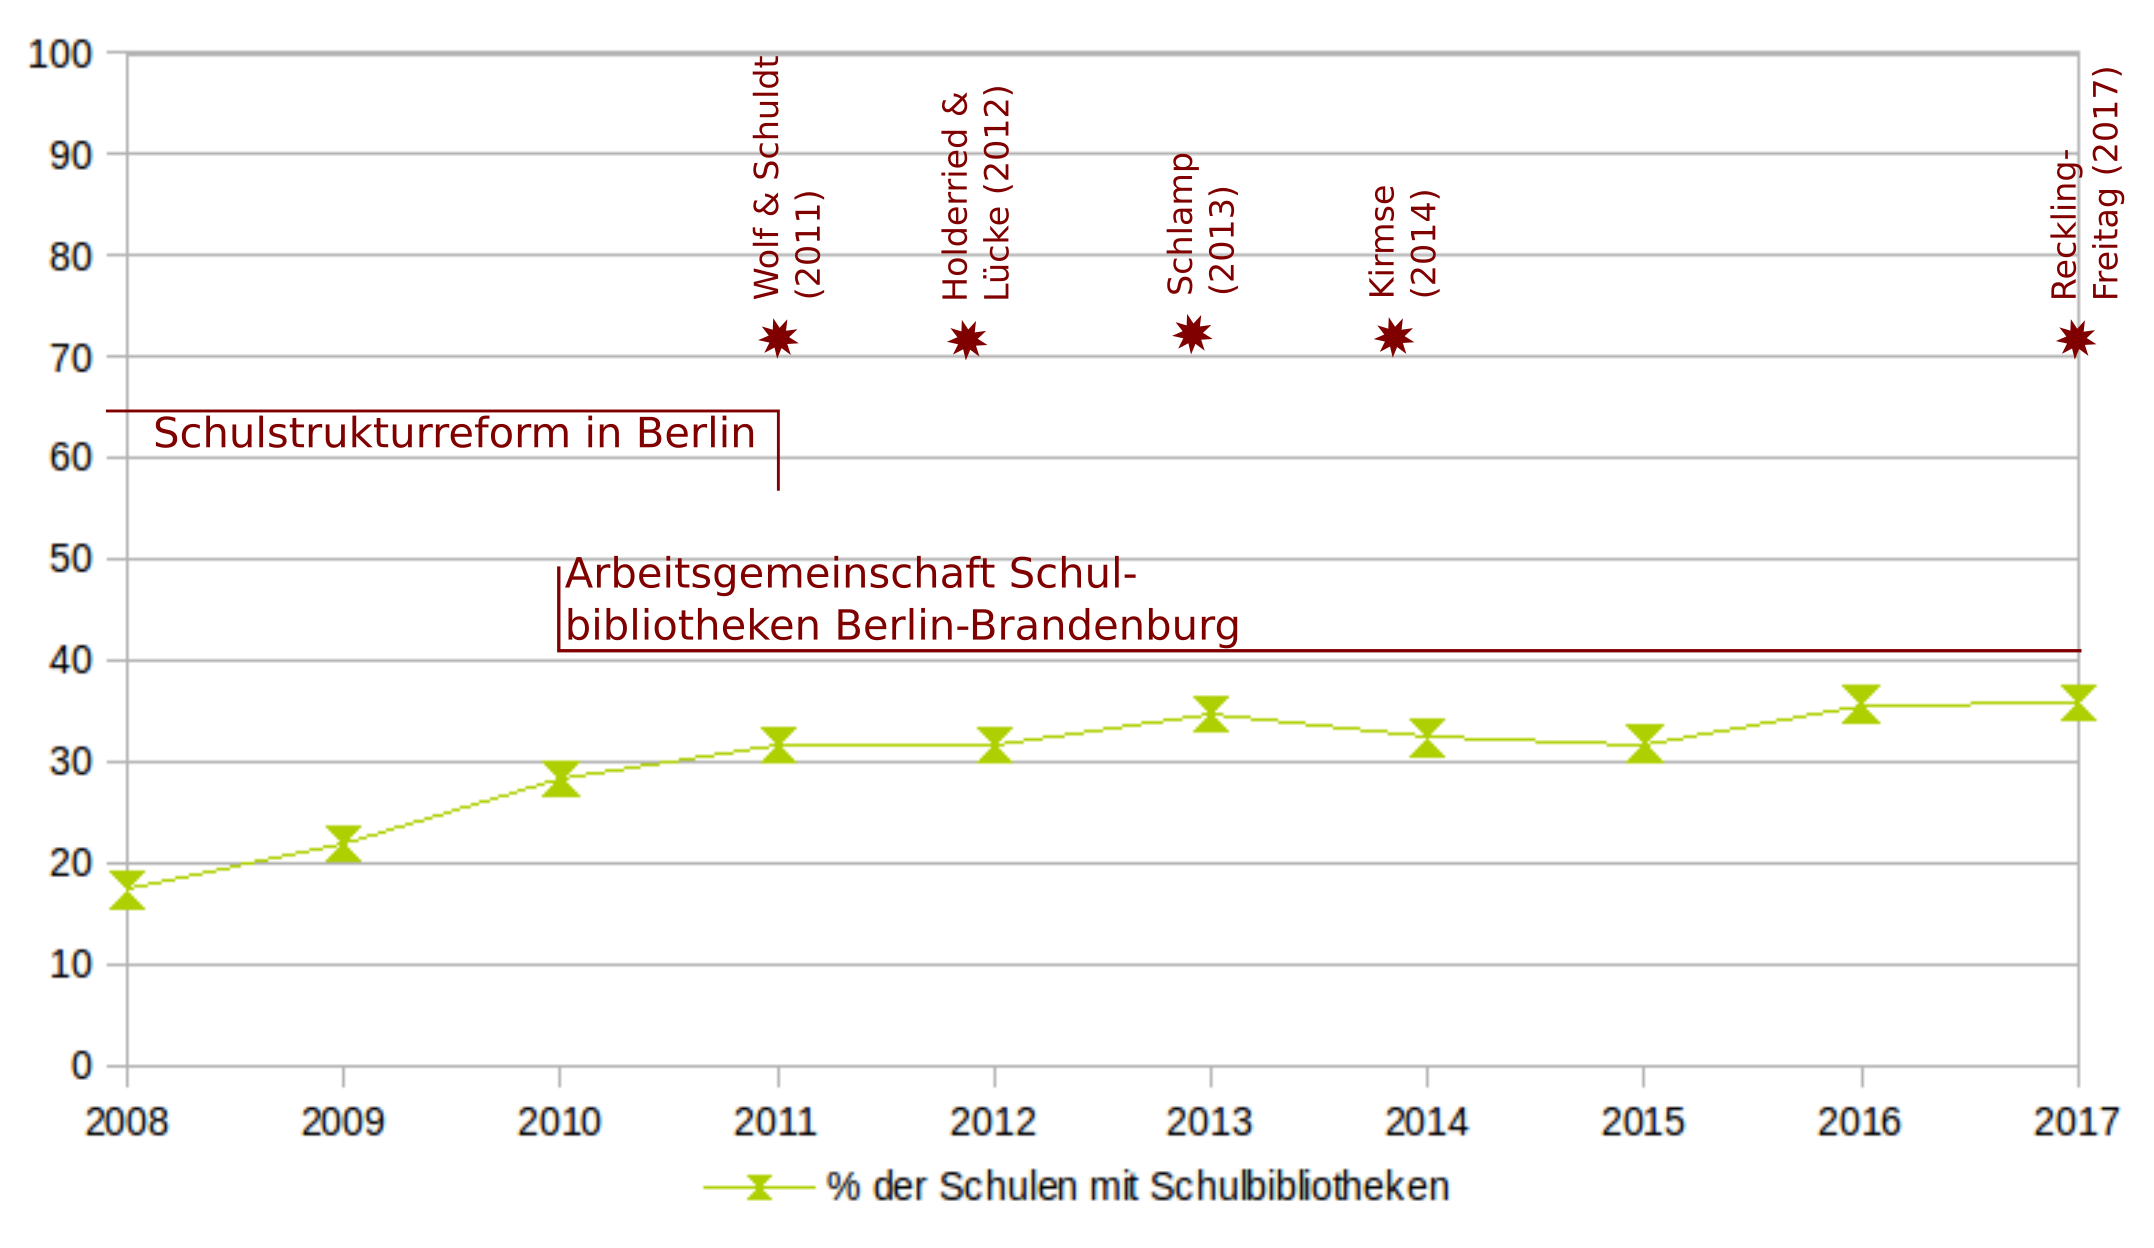
\includegraphics{img/abbildung.png}
\caption{Entwicklung der Schulbibliotheken inklusive der gerade
erwähnten Ereignisse}
\end{figure}

Bei all diesen Ereignissen wäre zu erwarten, dass es eine sichtbare
Veränderung der Zahl der Schulbibliotheken geben könnte: Schulen könnten
durch die Publikationen überzeugt werden, Bibliotheken einzurichten, ein
Interesse der ZLB könnte die Gründung von Schulbibliotheken
beschleunigen, die Wettbewerbe zur Schulbibliothek des Jahres könnten
diese sichtbar machen etc.

Der Eindruck ist aber ein ganz anderer: Die Schulstrukturreform und das
Wachstum der Zahl von Schulbibliotheken scheinen in einem Zusammenhang
zu stehen. Selbstverständlich ist diese Korrelation kein Beweis, aber es
lässt sich vermuten, dass die Aktivitäten in Schulen, welche auf die
Reformen folgten, auch dazu führten, dass Schulbibliotheken eingerichtet
wurden.

Die anderen Ereignisse scheinen keinen Einfluss gehabt zu haben.
Insbesondere bei den Publikationen scheint sogar, als seien sie
veröffentlicht worden, als das mögliche Interesse schon wieder verebbt
war (wobei nochmal darauf zu verweisen ist, dass weiterhin
Schulbibliotheken eröffnet, aber auch andere wieder geschlossen wurden;
eventuell sind die neuen also dennoch von den Publikationen motiviert
worden). Dies stellt zumindest die Hoffnungen auf ein weiteres Wachstum
der Zahl der Schulbibliotheken, die sich zum Beispiel offensichtlich bei
den Aktionen der Arbeitsgemeinschaft Schulbibliotheken
Berlin-Brandenburg gemacht werden, in Frage.

\section{Überprüfung der
Thesen}\label{uxfcberpruxfcfung-der-thesen}

Auf der präsentierten Datengrundlage können nun die zu Beginn der Studie
aufgestellten Thesen überprüft werden.

\textbf{These 1: Schulen mit Schulbibliotheken werden in Berlin auch in Zukunft
in der Minderheit bleiben.}

Diese These lässt sich leicht operationalisieren. Setzt man die
Minderheit der Schulen bei 50\% minus einer an, bestätigt sich die
These, wenn die Anzahl der Schulen in den Daten in den untersuchten zehn
Jahren nie diesen Wert überschreitet. Dies ist so eingetreten, nicht nur
bei der Gesamtheit der Schulen, sondern auch in allen einzelnen
Schulformen. Sicherlich könnte man die These weiter differenzieren und
zum Beispiel unterschiedlich starke Minderheiten einführen,
beispielsweise irrelevante Minderheiten von 0\%-10\%, relevante
Minderheiten bei 10\%-25\% und starke Minderheiten bei 25\%-50\%. Dann
würde sich zeigen, dass die Schulen mit Schulbibliotheken -- allerdings
nicht bei allen Schultypen -- zu einer starken Minderheit geworden sind.

Aber auch dies würde nicht bedeuten, dass der Eindruck entstünde, dass
die Schulen mit Schulbibliotheken in absehbarer Zeit mehr als 50\% der
Schulen in Berlin ausmachen würden. Vielmehr scheint die dynamische
Entwicklung vorbei zu sein. (Wieder bezogen auf die Gesamtheit der
Schulen, in einzelnen Schulen hingegen scheint es immer wieder zum
Aufbau, Umbau und der Schliessung von Schulbibliotheken zu kommen.)
Vielmehr scheint die These auch für die absehbare Zukunft aufgestellt
werden zu können, falls es nicht zu radikalen Veränderungen in der
Schul- oder Bibliothekspolitik kommen sollte.

These 1 ist somit bestätigt.

\textbf{These 2: In Bezug auf Schulbibliotheken bleiben die Gymnasien den
anderen Schulen mit Sekundarstufen gegenüber überausgestattet.}

Auch diese These lässt sich leicht operationalisieren. Sie wird gültig,
wenn Schulen mit Sekundarstufe (bis 2010/2011 Haupt-, Real- und
Gesamtschulen; ab 2010/2011 Integrierte Sekundarschulen, durchgängig die
Freien Waldorfschulen) in jedem Jahr weniger Schulbibliotheken auswiesen
als die Gymnasien. Dies ist so eingetreten. Teilweise war die
Wahrscheinlichkeit, in einem Berliner Gymnasium eine Schulbibliothek
vorzufinden, doppelt so hoch, wie in den Integrierten Sekundarschulen.
Unter den Haupt- und Realschulen sowie Freien Waldorfschulen waren die
Schulen mit Schulbibliothek offenbar immer eine Seltenheit. Wenn man
davon ausgeht -- zumindest tut dies die bibliothekarische Literatur zu
Schulbibliotheken --, dass Schulbibliotheken zum Schulerfolg beitragen,
stellt dieses Ergebnis eigentlich den grössten Skandal dar, der sich in
den gesammelten Daten findet. Offenbar haben in Berlin die Schülerinnen
und Schüler der Gymnasien, die ehedem schon privilegiert sind, auch
einen privilegierten Zugang zu Schulbibliotheken. Nicht alle, aber doch
viel mehr, als die Schülerinnen und Schüler anderer
Schulformen.\footnote{Für die Freien Waldorfschulen liesse sich
  vielleicht argumentieren, dass die dortigen Schülerinnen und Schüler
  anders (ökonomisch) privilegiert seien; aber dies würde nur für eine
  relativ kleine Zahl von Kindern und Jugendlichen gelten.}

These 2 ist somit bestätigt.

\textbf{These 3: Die Schulstrukturreform wird kurzfristig zu einem Anstieg der
Zahl von Schulbibliotheken führen, die mittelfristig wieder auf das
Niveau vor der Reform sinken wird.}

\textbf{These 3a: Dies wird insbesondere für die neu geschaffene Schulform
Integrierte Sekundarschule gelten.}

Diese These sagt eine Kurve in den Daten voraus. Die Zahl der
Schulbibliotheken müsste 2010/2011 mit der Schaffung der Integrierten
Sekundarschulen massiv steigen, dann bis zum Ende des
Untersuchungszeitraums (2017) wieder auf eine Niveau wie 2008/2009
sinken. Die Daten zeigen eine andere Entwicklung. Zwischen 2008 und 2012
hat sich die Zahl der Schulen mit Schulbibliotheken in Berlin massiv
erhöht. Im Sinne der These lässt sich, wie schon diskutiert, hier ein
Zusammenhang mit der Schulstrukturreform vermuten.

Allerdings ist die Zahl seitdem nicht mehr massiv gesunken, sondern
verblieb auf diesem Niveau von ungefähr einem Drittel der Schulen. Zu
vermuten ist, dass die Schulstrukturreform tatsächlich mehr Aktivitäten
in den Schulen auslöste, unter anderem in Bezug auf Schulbibliotheken,
als in der These erwartet wurde.

In Bezug auf Integrierte Sekundarschulen hätte die These genauer
formuliert werden müssen. Im Vergleich zu den drei Schulformen, aus der
sie entstanden ist, gab es 2011 weit mehr Schulbibliotheken als in den
Haupt- und Realschulen, aber weniger als in den Gesamtschulen.
Angesichts dessen, dass es auch mehr Haupt- und Realschulen als
Gesamtschulen gab, kann von einem Anstieg der Zahl der Schulbibliotheken
gesprochen werden, allerdings keinem eindeutigen. Gleichzeitig
entwickelte sich die Zahl in den folgenden Jahren auf diesem Niveau
weiter und ging nicht auf das niedrige Niveau der Haupt- und Realschulen
zurück.

Insoweit lässt sich sagen, dass die These richtig den Anstieg von
Schulbibliotheken voraussagte, aber viel zu negativ in Bezug auf die
weitere Entwicklung war.

These 3 ist somit in grossen Teilen widerlegt.

These 3a ist ebenfalls zu grossen Teilen widerlegt.

\textbf{These 4: Die Bibliotheken in Schulen werden weiterhin hauptsächlich als
\enquote{Lesebibliotheken} verstanden und genutzt.}

Diese These basiert auf den Erfahrungen aus der weiter oben genannten
Magisterarbeit (Schuldt 2006), die unter anderem Besuche in
Schulbibliotheken beinhaltete. Dies liess sich 2017 aufgrund beruflicher
Verpflichtungen des Autors nicht reproduzieren. Es muss zur
Operationalisierung also auf die Darstellung der Schulbibliotheken
selber zurückgegriffen werden. Dazu wurden die Darstellungen der
Schulbibliotheken, die sich 2017 finden liessen, inhaltlich ausgewertet.
Genutzt wurden dazu die Modelle von Schulbibliotheken, die 2010 auf der
Basis der damals vorliegenden Daten gebildet wurden. (Schuldt
2010:12-14) und seitdem mehrfach anderswo Verwendung fanden (Holderried
\& Lücke 2012; Wolf \& Schuldt 2011; Rega 2015), also offenbar eine
gewisse Überzeugungskraft haben.

\begin{enumerate}
\def\labelenumi{\arabic{enumi}.}
\item
  Schulbibliotheken als Orte des guten Unterrichts
\item
  Schulbibliotheken als Lese-Lern-Räume
\item
  Schulbibliotheken als Offene Lernräume
\item
  Schulbibliotheken als schulfreie Räume in Schulen
\item
  Schulbibliotheken als kleine Stadtteilbibliotheken
\end{enumerate}

Es wurde versucht, die vorgefundenen Schulbibliotheken jeweils einem
Modell zuzuordnen. Die Datenbasis ist gering, da die meisten Schulen
ihre Schulbibliotheken, wie schon erwähnt, nicht wirklich beschrieben.
Es ergibt sich aber folgendes Bild:

\begin{longtable}[]{@{}lr@{}}
\caption*{Tabelle 4: Modelle und Zahl der Schulbibliotheken, die sich zuordnen
lassen}\tabularnewline
\toprule
\begin{minipage}[b]{0.41\columnwidth}\raggedright\strut
Modell der Schulbibliothek\strut
\end{minipage} & \begin{minipage}[b]{0.41\columnwidth}\raggedleft\strut
Anzahl Schulbibliothek (2017)\strut
\end{minipage}\tabularnewline
\midrule
\endfirsthead
\toprule
\begin{minipage}[b]{0.41\columnwidth}\raggedright\strut
Modell der Schulbibliothek\strut
\end{minipage} & \begin{minipage}[b]{0.41\columnwidth}\raggedleft\strut
Anzahl Schulbibliothek (2017)\strut
\end{minipage}\tabularnewline
\midrule
\endhead
\begin{minipage}[t]{0.41\columnwidth}\raggedright\strut
Schulbibliotheken als Orte des guten Unterrichts\strut
\end{minipage} & \begin{minipage}[t]{0.41\columnwidth}\raggedleft\strut
0\strut
\end{minipage}\tabularnewline
\begin{minipage}[t]{0.41\columnwidth}\raggedright\strut
Schulbibliotheken als Lese-Lern-Räume\strut
\end{minipage} & \begin{minipage}[t]{0.41\columnwidth}\raggedleft\strut
31\strut
\end{minipage}\tabularnewline
\begin{minipage}[t]{0.41\columnwidth}\raggedright\strut
Schulbibliotheken als Offene Lernräume\strut
\end{minipage} & \begin{minipage}[t]{0.41\columnwidth}\raggedleft\strut
16\strut
\end{minipage}\tabularnewline
\begin{minipage}[t]{0.41\columnwidth}\raggedright\strut
Schulbibliotheken als schulfreie Räume in Schulen\strut
\end{minipage} & \begin{minipage}[t]{0.41\columnwidth}\raggedleft\strut
5\strut
\end{minipage}\tabularnewline
\begin{minipage}[t]{0.41\columnwidth}\raggedright\strut
Schulbibliotheken als kleine Stadtteilbibliotheken\strut
\end{minipage} & \begin{minipage}[t]{0.41\columnwidth}\raggedleft\strut
3\strut
\end{minipage}\tabularnewline
\bottomrule
\end{longtable}

Dieses Ergebnis gleichen den 2006 gewonnenen Eindrücken. Schulen
orientieren sich nicht an bibliothekarischen Modellen (obwohl sie es
heute durch die schon genannten Monographien zu Schulbibliotheken
einfacher könnten als 2006), sondern verstehen Schulbibliotheken vor
allem als Orte des Lesens, des freien Lernens und der
Freizeitgestaltung.\footnote{Ein Beispiel für die Diskrepanzen zwischen
  bibliothekarischen Vorstellungen, die Schulbibliotheken als Zentrum
  der Schule verstehen, und Vorstellungen von Schulbibliotheken, wie sie
  in den Schulen verbreitet zu sein scheinen, bietet die Grundschule am
  Koppenplatz (2017), die über ihre Bibliothek schreibt: \enquote{Die
  Bibliothek ist ein Raum der Stille. Ein Rückzugsort für Kinder, wo sie
  in Regalen nach Büchern stöbern und sich in eine gemütliche Ecke
  zurückziehen können.}} Von den drei Schulbibliotheken, die sich eher
an bibliothekarischen Vorstellungen zu orientieren scheinen (Carl von
Ossietzky Schule, Gottfried-Keller Gymnasium, Französisches Gymnasium /
Lycée Français de Berlin), bezieht sich das Lycée Français de Berlin
offenbar auf die Vorbilder in französischen Schulen (so heisst die
Einrichtung auch, wie in Frankreich, Centre de documentation et
d'information (CDI)) und nicht auf das deutsche Bibliothekswesen.
Entgegen aller Vorschläge scheinen Schulbibliotheken in Berlin auch kaum
als Unterrichtsort genutzt zu werden.

These 4 ist damit bestätigt, allerdings auf einer sehr kleine
Datenbasis.

\textbf{These 5: Der Grossteil der Schulbibliotheken in Berlin wird
diskontinuierlich betrieben.}

Diese These wurde so operationalisiert, das eine Schulbibliothek als
kontinuierlich betrieben galt, wenn sie drei oder mehr Jahre
nacheinander betrieben wurde. Im Idealfall würde sie einmal gegründet
und dann die gesamte Zeit über, in der die Schule existiert, betrieben
werden. Deshalb wurde die Aussage so gefasst: eine Schulbibliothek gilt
als kontinuierlich betrieben, wenn sie seit mindestens drei Jahren
nachzuweisen ist und 2017 existiert. Aufgrund der Datenlage wurde
akzeptiert, wenn sie innerhalb ihrer Existenz eine Jahr lang nicht
nachgewiesen werden konnte, aber zuvor und danach, da dies eher auf die
Aktualität der jeweiligen Schulhomepage und weniger auf die
Schulbibliothek selber zurückgeführt werden kann. Ansonsten, also wenn
sie zwei oder mehr Jahre lang nicht nachgewiesen wurde, galt sie als
geschlossen. Die These wäre widerlegt, wenn 50\% plus 1 Schulbibliothek
als kontinuierlich betreiben gelten könnte. Wie schon dargestellt
(Abschnitt 3, Tabelle 3) trifft dies knapp zu.

Gleichwohl, das wurde auch schon dargestellt, ist die Landschaft der
Schulbibliotheken in Berlin weiterhin stark dynamisch (45,8\% der
Schulbibliotheken, die 2017 nachzuweisen waren, wurden offenbar 2016
oder 2017 eröffnet). Für eine Fortführung des Projektes müsste die These
wohl differenzierter gefasst werden.

These 5 ist widerlegt.

\textbf{6. These: Die neue Literatur zu Schulbibliotheken, die
Arbeitsgemeinschaft Schulbibliotheken Berlin-Brandenburg sowie die
Stelle für schulbibliothekarische Arbeit in Treptow-Köpenick werden sich
in einer steigenden Anzahl von Schulbibliotheken in Berlin sowie in
Schulbibliotheken, die sich eher am \enquote{bibliothekarischen Modell}
orientieren, niederschlagen.}

Diese These lässt sich schwieriger operationalisieren, da die Einflüsse
von Bibliotheken oder die Arbeit der Arbeitsgemeinschaft
Schulbibliotheken Berlin-Brandenburg sich eventuell erst zwei oder drei
Jahre später in den erhobenen Daten zeigen könnten. Insoweit wäre ein
Abschätzung notwendig. Zieht man allerdings die weiter oben (Abschnitt
3.2) dargestellte Graphik (Graphik 1) heran, auf der für
Schulbibliotheken eventuell wirksame Ereignisse gegenüber der
Entwicklung der Zahl der Schulbibliotheken in Berlin abgetragen wurden,
lässt sich festhalten, dass die Ereignisse keinen sichtbaren Einfluss
auf die Zahl der Schulbibliotheken hatten, weder kurz- noch
mittelfristig. Einzig die Gründung der Arbeitsgemeinschaft im Jahre 2010
scheint mit dem Anstieg der Zahl von Schulbibliotheken in Verbindung zu
stehen. Zu vermuten ist allerdings, auch weil die weiteren Aktivitäten
der Arbeitsgemeinschaft keinen nachweisbaren Effekt hatten, dass eher
andersherum das rasante Wachstum, das heisst vor allem die vielen
Neugründungen von Schulbibliotheken, zur Gründung der
Arbeitsgemeinschaft führten, da auf einmal genügend Personen an der
Arbeit von Schulbibliotheken interessiert waren und sich zusammenfanden.

These 6 ist somit auch widerlegt.

\section{Diskussion der
Ergebnisse}\label{diskussion-der-ergebnisse}

Die erhobenen Daten und geprüften Thesen zeigen eine Entwicklung von
Schulbibliotheken, die von den einzelnen Schulen bestimmt zu sein
scheint und auf die direkt wenig Einfluss genommen werden kann.

Sichtbar wurden zwei Trends. Erstens: Ein Grossteil der Schulen in
Berlin kommt weiterhin ohne Schulbibliothek aus; es sind zudem
wiederholt Schließungen zu verzeichnen. Das widerspricht Erwartungen,
die sich in der bibliothekarischen Literatur gemacht werden. In dieser
wird postuliert, dass gute Schulbibliotheken zum zentralen Ort von
Schulen würden und -- implizit in der Literatur, aber explizit in
Projekten, die Modell-Schulbibliotheken gründen und hoffen, dass diese
als Vorbilder zur Gründung weiterer Schulbibliotheken führen (Schuldt
2012) -- eine Auswirkung auf andere Schulen hätten. Dies scheint den
Eindruck zu bestätigen, dass es nicht die bibliothekarischen
Vorstellungen, sondern die Entscheidungen in den einzelnen Schulen --
die auch auf Vorstellungen und Annahmen beruhen -- sind, welche
erklären, ob und in welcher Form Schulbibliotheken eingerichtet oder
unterhalten werden. (Schuldt, Mumenthaler \& Vardanyan 2016) Besonders
auffällig ist dies, da Schulen in Berlin im Rahmen der Schulreform mehr
Autonomie in Bezug auf Etat und Personal erhalten haben, die sie für
andere Schulbereiche auch nutzen, und aus der heraus sie
Schulbibliotheken mit bibliothekarisch ausgebildetem Personal schaffen
könnten, wie das in der bibliothekarischen Literatur (oder von der
Arbeitsgemeinschaft Schulbibliotheken Berlin-Brandenburg (2017))
vorgeschlagen wird. Diese Vorschläge scheinen Schulen aber nicht zu
überzeugen.

Zweitens: Den grössten Einfluss auf die Zahl der Schulbibliotheken hatte
offenbar die Schulstrukturreform in Berlin, die in Schulen
Veränderungsprozesse anregte, die sich auch in der verstärkten Gründung
von Schulbibliotheken niederschlug. Diese Reform griff in das
Selbstverständnis der Schulen ein und forderte sie auf, sich
eigenständig weiterzuentwickeln. Eine Idee, die oft auftauchte --
beispielsweise in den Schulprogrammen, die jede Schule anfertigen muss
--, scheint die zu sein, eine Schulbibliothek einzurichten. Andere
mögliche Interventionen in Bezug auf Schulbibliotheken hatten offenbar
keinen direkten Einfluss, zumindest nicht auf die Zahl der
Schulbibliotheken und auch nicht wirklich sichtbar auf deren
Vorstellungen davon, was Schulbibliotheken sein sollen.\footnote{Dabei
  muss angemerkt werden, dass aus den bezirklichen Bibliothekssystemen
  und der ZLB kaum wahrnehmbare Aktivitäten in Richtung
  Schulbibliotheken entfaltet werden. Diese sind, wenn, dann eher
  ausserhalb der Sichtbarkeit verlaufen. Einzig im Bezirk Spandau
  unterstützt die Öffentliche Bibliothek eine Zahl von Schulen direkt.
  (Siehe zum Beispiel Grundschule am Weinmeisterhorn (2017).) Das schon
  angesprochene Projekt, eine schulbibliothekarische Arbeitsstelle an
  der ZLB zu errichten (Arbeitsgemeinschaft Schulbibliotheken
  Berlin-Brandenburg 2013), scheint keine Ergebnisse erbracht zu haben.
  Die Stelle für schulbibliothekarische Arbeit im Bezirk
  Treptow-Köpenick ist beim Schulamt angesiedelt.} Es ist die
Schulpolitik, die einen übergreifenden Einfluss hat und dann die lokale
Schulgemeinschaft selber, die Schulbibliotheken einrichtet, unterhält,
nutzt oder auch wieder schliesst. Andere Einflüsse scheinen, wenn
überhaupt, nur begrenzt lokal wirksam gewesen zu sein. Diese Erkenntnis
-- die sich auch mit Ergebnissen anderer Projekte deckt (Schuldt 2012),
aber hier anhand von Daten nochmal untermauert wurde -- sollte in allen
weiteren Diskussionen über und Projekten zu Schulbibliotheken beachtet
werden.

Weiterhin -- um die Ergebnisse auch positiv zu deuten -- wurde sichtbar,
dass es Schulbibliotheken in Berlin gibt und zwar in beachtlicher Zahl,
die zudem -- da es kaum finanzierte Stellen zu geben scheint -- von
einer beachtlichen Zahl von ehrenamtlich oder zumindest, bei
Lehrpersonen, über ihre Anstellung hinaus engagierten Personen betrieben
werden.\footnote{Selbstverständlich werden die Anstellungsverhältnisse
  des Personals nicht regelmässig auf den Homepages der Schulen
  dargestellt, insoweit basiert diese Aussage auf Erfahrungen aus den
  Schulbibliotheken selber und auf Hinweisen aus den Darstellungen. Auf
  eine bibliothekarische Ausbildung des Personals wird aber nie
  hingewiesen, eher schon auf das Ehrenamt oder aber, selten, auf
  Personal, dass im Rahmen des Bundesfreiwilligendienstes (seit 2011)
  angestellt ist (was selbstverständlich für Schulbibliotheken, die
  kontinuierlich arbeiten sollen, nicht optimal ist, da diese Personen
  im Normalfall für 12 Monate angestellt sind, nicht jedes Mal ein
  Ersatz garantiert ist und sie vor allem nur in \enquote{zusätzlichen
  Projekten} -- also nicht dem Kern der Arbeit einer Institution --
  arbeiten dürfen, was auch heisst, dass die jeweiligen
  Schulbibliotheken nicht als zum Kern der jeweiligen Schule -- wie das
  die bibliothekarische Literatur vorschlägt -- gezählt werden).}

Zudem zeigt sich zwar eine grosse Dynamik, aber auch ein Kern von
Schulbibliotheken (sowie die auf Dauer gestellte Arbeitsgemeinschaft
Schulbibliotheken Berlin-Brandenburg), die Schulbibliotheken nicht als
Experimente oder Aufbauprojekte betreiben wollen, sondern als
langfristig etablierte Einrichtungen. In diesen Einrichtungen werden
Erfahrungen darüber gesammelt, wie Schulbibliotheken in Berliner Schulen
tatsächlich funktionieren, was sie tatsächlich benötigen um bestimmte
Funktionen zu erfüllen, welche Vorstellungen -- zum Beispiel von
bibliothekarischer Seite -- überzeugend sind und welche nicht. Sowohl
praktische Vorschläge für Schulbibliotheken und ihren Betrieb als auch
eine Theorie, die dies beschreiben will, könnte auf diese Erfahrungen
aufbauen. Das scheint bisher kaum und wenn, dann eher im persönlichen
Kontakt (wie über die Stelle für schulbibliothekarische Arbeit in
Treptow-Köpenick, die innerhalb des Bezirks den Erfahrungsaustausch
organisiert oder teilweise die Schulbibliothekstage der
Arbeitsgemeinschaft Schulbibliotheken Berlin-Brandenburg) zu
geschehen.\footnote{Man könnte erwarten, dass die Arbeitsgemeinschaft
  Schulbibliotheken Berlin-Brandenburg diese Aufgabe mehr übernimmt.
  Aber, zum Beispiel, deren Broschüre, die vorbildhafte
  Schulbibliotheken präsentieren soll (Arbeitsgemeinschaft
  Schulbibliotheken Berlin-Brandenburg 2013), besteht eigentlich nur aus
  unverbindlichen, übermässig positiven Darstellungen, ihre weiteren
  Texte (Arbeitsgemeinschaft Schulbibliotheken Berlin-Brandenburg 2017;
  Hardtke-Flodell, Frübing \& Wolter 2013, aber auch der Blog der
  Arbeitsgemeinschaft auf ihrer Homepage
  \url{http://schulbibliotheken-berlin-brandenburg.de}) reproduzieren
  relativ unkritisch bibliothekarische Vorstellungen, so dass zum Teil
  der Eindruck entsteht, als hätten die konkreten Erfahrungen aus den
  konkreten Bibliothek in Berliner Schulen keinen Einfluss.}

Zu beachten sind auch die Kontinuitäten, die sich während der
Datensammlung zeigten. Schulbibliotheken werden über die ganzen Jahre
hinweg zumeist als Anstrich bei der Aufzählung der Schulausstattungen
aufgezählt und nur in einigen Fällen von der Schulgemeinschaft als so
wichtig angesehen, dass sie mehr Platz auf der Homepage erhalten. Es gab
Ausnahmen, bei denen Schulbibliotheken zum Beispiel eigene Homepages
erhielten. Aber für die meisten Schulen scheinen sie den Status von
Unterstützungseinrichtungen zu haben. Zudem werden Schulbibliotheken
weiterhin nicht nach bibliothekarischen Vorstellungen (also
beispielsweise mit Katalog, aktiver Bestandspolitik, Medienmix,
bibliothekarisch ausgebildetem Personal) betrieben, sondern als Lese-
und Freizeitraum. Dies hat sich zwischen 2008 und 2017 nicht verändert.

\section{Welche Bedeutung haben die Ergebnisse für das
bibliothekarische Denken über
Schulbibliotheken?}\label{welche-bedeutung-haben-die-ergebnisse-fuxfcr-das-bibliothekarische-denken-uxfcber-schulbibliotheken}

Die Ergebnisse dieses Projektes könnten auch in der Schulforschung von
Bedeutung sein. Dies wäre aber von den Erziehungswissenschaften zu
klären. Für das Bibliothekswesen (und die Bibliothekswissenschaft) ist
es für den Autor (als Bibliotheks- und nicht Erziehungswissenschaftler)
aber möglich, einige Aussagen zu machen.

\begin{enumerate}
\def\labelenumi{\arabic{enumi}.}
\item
  Seit den 1970er Jahren hat sich in den deutschsprachigen
  Bibliothekswesen (also Deutschland, Österreich, Schweiz) eine
  bestimmte Vorstellung von Schulbibliotheken etabliert, insbesondere
  dazu, wie sie aufzubauen, zu führen und zu nutzen seinen. Diese
  Vorstellungen schlagen sich in den bibliothekarischen Publikationen zu
  Schulbibliotheken nieder (unter anderem Holderried \& Lücke 2011;
  Kremske 2013; in der Schweiz als Richtlinien: Schweizerische
  Arbeitsgemeinschaft der allgemeinen öffentlichen Bibliotheken
  2014).\footnote{Mehrfach wurde in diesem Text erwähnt, dass die
    bibliothekarischen Texte seit den 1970er Jahren diese Vorstellungen
    von Schulbibliotheken als \enquote{kleine Öffentliche Bibliotheken}
    vertreten. Es ist möglich, eine Traditionslinie zum Buch von Doderer
    et al. (1970) aufzuzeigen, welches diese Forderung zuerst im
    modernen Bibliothekswesen erhob. Vereinzelt fanden sich solche
    Vorstellungen aber auch schon vorher, zum Beispiel -- im Anschluss
    an den Erlass des Ministern für Wissenschaft, Kunst und Volksbildung
    in Preussen von 1928 zur \enquote{Neugestaltungen und Auswertung der
    Schülerbüchereien in den Volksschulen} in der späten Weimarer
    Republik -- bei Schulz \& Sielaff (1930).} Mit diesen Vorstellungen
  geht auch der -- mal mehr und mal weniger direkt formulierte --
  Anspruch einher, den Schulen diese Vorstellungen als modern oder
  zeitgemäss vorgeben zu können. (Auch die Arbeitsgemeinschaft
  Schulbibliotheken Berlin-Brandenburg (2017) scheint aktuell diesen
  Diskurs zu übernehmen.) Die Ergebnisse des Projektes zeigen, dass in
  den Schulen diese Vorstellungen nicht wahr- oder angenommen zu werden
  scheinen (siehe auch Schuldt, Mumenthaler \& Vardanyan (2016), wo sich
  dies ebenso in den Volksschulen des Kantons St.~Gallen zeigte) und der
  Einfluss der bibliothekarischen Interventionen nicht nachzuweisen ist.
  Die schon einmal vom Autor aufgestellte Forderung (Schuldt 2012), die
  Vorstellungen von Schulbibliotheken, die im Bibliothekswesen
  verbreitet sind, zu überdenken und vor allem nicht (mehr) als
  alternativlos darzustellen, wurde von diesen Ergebnissen nur weiter
  untermauert.
\item
  Gleichzeitig zeigten die Ergebnisse auch in Schulen ein ständig
  wiederkehrendes Interesse an Schulbibliotheken, auf das reagiert
  werden könnte. Die Schulen warten nicht unbedingt darauf, dass
  Öffentliche Bibliotheken sie anleiten. Vielmehr haben sie eigene
  Vorstellungen davon, wie ihre Bibliotheken sein sollten und entwickeln
  wohl auch eigene Abläufe in den Schulbibliotheken. Das heisst aber
  nicht, dass sie nicht bestimmte Unterstützungen wünschen würden. Das
  Potential ist offenbar vorhanden. Dafür wäre es aber nötig, dass das
  Öffentliche Bibliothekswesen die Eigenheiten der Schulbibliotheken zu
  verstehen lernt und diese als eigenständige Bibliotheksform -- und
  nicht als Sonderform Öffentlicher Bibliotheken -- akzeptiert. Dies
  wäre dann auch politisch einklagbar, Forderungen nach Mitteln und
  Personal wären so gut zu untermauern, wenn es nicht wieder (Schuldt
  2012) darum gehen sollte, die Schulen auf ein bibliothekarisches
  Verständnis von Schulbibliotheken einzuschwören, sondern sie bei lokal
  aufkommenden Fragen zu unterstützen.\footnote{Ein Thema, dass sich
    immer wieder aufdrängt, ist das Bestehen des Bibliothekswesens
    darauf, dass eine Schulbibliothek einen Katalog als
    Nachweisinstrument nach bibliothekarischen Regeln zu führen hätte,
    wie dies Öffentliche Bibliotheken auch tun (schon bei Schulz \&
    Sielaff (1930) und bei Doderer et al. (1970), aber auch Kirmse
    (2014) und Arbeitsgemeinschaft Schulbibliotheken Berlin-Brandenburg
    (2017)), während es wenig Hinweise darauf gibt, dass
    Schulbibliotheken dies wünschen (zum Beispiel führte keine der in
    der Magisterarbeit (Schuldt 2006) besuchten Schulbibliotheken einen,
    auch nicht die in einer anderen Studie (Schuldt, Mumenthaler \&
    Vardanyan 2016) besuchten Schulbibliotheken im Kanton St.~Gallen).
    Dementsprechend führen nur sehr wenige der in Berlin zu findenen
    Schulbibliotheken einen Katalog, noch weniger als
    Nachweisinstrument.} Ein Thema, welches dabei mit einbezogen werden
  müsste, ist die Tendenz, Schulbibliotheken nicht per se als
  Einrichtungen auf Dauer zu stellen. (Ein Grund dafür könnte sein, dass
  deren Existenz auf dem Ehrenamt Einzelner basiert, die irgendwann die
  Schule verlassen.) Bibliothekarische Texte gehen oft davon aus, dass
  sie kontinuierlich betrieben werden müssten, das ist in den Schulen
  nicht per se so ausgemacht, sondern nur teilweise, und wird sich als
  Situation ohne eine Änderung der Schulpolitik auch nicht ändern.
\item
  Schulbibliotheken müssen als eigenständige Einrichtungen verstanden
  werden, die vor allem von der jeweiligen Schulgemeinschaft und den
  Interessen der in ihr Aktiven bestimmt werden. Dies wird sich wohl
  auch nicht ändern, solange sich Schul- und Bibliothekspolitik nicht
  ändern. Andere Interventionen (Handbücher, Schulbibliothekstage,
  Arbeitsgemeinschaft Schulbibliotheken) scheinen immer nur einen
  begrenzten oder keinen Einfluss zu haben, zumindest in Bezug auf die
  Zahl der Schulbibliotheken.
\item
  Für die Bibliothekswissenschaft stellen sich interessante Fragen. So
  ist es weiterhin nicht geklärt, wie und wann Schulen sich entscheiden
  -- und wer genau in der jeweiligen Schulgemeinschaft diese
  Entscheidung trifft --, Schulbibliotheken zu gründen, umzubauen und
  wieder zu schliessen. Zu klären wäre, was sich Schulen von diesen
  ständigen Neugründungen versprechen. Weiterhin offen bleibt auch, was
  Schulbibliotheken im Schulalltag tatsächlich für Wirkungen haben,
  insbesondere bei den Schülerinnen und Schülern. Die bibliothekarische
  Literatur enthält zu dieser Frage zwar immer wieder weitreichende
  (aber auch seit einigen Jahrzehnten kaum veränderte) Vermutungen, die
  vor allem auf einem Modell von Schulbibliotheken aufbauen, dass sich,
  wie dargestellt, praktisch nicht findet. Deshalb sind diese
  Vorstellungen für die Frage nach der tatsächlichen Wirkung wenig
  hilfreich. Es wäre sinnvoll, diese zu erfassen, um das
  bibliothekarische Denken über Schulbibliotheken eher an der Realität
  zu orientieren.
\item
  Eine wichtige Frage, egal für welche Forschungsrichtung, ist die
  danach, welchen Effekt die Ungleichverteilung von Schulbibliotheken
  zwischen den Schulformen hat; ob diese Effekte gewollt sind und wenn
  nicht, wie diesen entgegenzuwirken wäre. In Grundschulen stellt sich
  gesondert die Fragen, wie insbesondere das Lesenlernen, dass oft als
  Grund für die Schulbibliotheken genannt wird, organisiert ist, wenn
  nicht mit der Schulbibliothek. Wieso haben eine sehr grosse Anzahl von
  Grundschulen in Berlin heute eine Schulbibliothek, aber eine noch
  grössere Anzahl nicht, wenn das Ziel -- das Lesenlernen zu ermöglichen
  -- in allen gleich ist?\footnote{Eine persönlich den Autor drängende
    Frage ist, wieso gerade die Bücherwurm Grundschule am Weiher in
    Marzahn-Hellersdorf offenbar seit zehn Jahren ohne Schulbibliothek
    auskommt. Wie motiviert sich sonst dieser Name?} In Bezug auf
  Gymnasien und Integrierte Sekundarschulen liegt die Vermutung nahe,
  dass die Schülerinnen und Schüler auf Gymnasien weiterhin privilegiert
  werden; aber eventuell haben Integrierte Sekundarschulen -- die auch
  zum Abitur führen -- andere Wege gefunden, um die gleichen Ziele zu
  erreichen, die Gymnasien eher mit Schulbibliotheken erreichen. Um das
  zu klären, wäre es selbstverständlich erst nötig zu klären, welche
  Ziele dies sind.
\end{enumerate}

\section{Fazit}\label{fazit}

In diesem Text wurde ein Projekt zur Entwicklung der Anzahl von
Schulbibliotheken in Berlin und ihrer Verteilung über die verschiedenen
Schulformen vorgestellt. Das Projekt basierte auf Thesen, die inhaltlich
von der restlichen bibliothekarischen Literatur über Schulbibliotheken
und den dort erhofften Entwicklungen abweicht.

Das Projekt konnte zeigen, dass mit einer realistischen Betrachtung der
Situation von Schulbibliotheken viele ihre Entwicklungen vorhergesagt
werden können. Vor allem aber zeigte sich, dass die Entwicklung von
Schulbibliotheken in Berlin und damit wohl auch grundsätzlich in
Deutschland -- obwohl es zum Beispiel in Bayern und Rheinland-Pfalz mehr
sichtbares Engagement des Öffentlichen Bibliothekswesens für
Schulbibliotheken gibt -- vor allem von den Schulen selber und der
Schulpolitik beeinflusst werden, nicht von bibliothekarischen
Vorstellungen. Sie müssen als eigenständiger Bibliothekstyp verstanden
werden.

Ein wichtiger Punkt, der durch das Projekt klar wurde, ist, dass jedes
Nachdenken darüber, ob und wie Öffentliche Bibliotheken und
Schulbibliotheken aufeinander zu beziehen sind, ob und welche
Unterstützung geleistet werden kann oder soll, auch welche Fragen zum
Beispiel in immer wieder neu angegangenen Abschlussarbeiten
bibliothekarischer Ausbildungsgänge über Schulbibliotheken gestellt
werden, sich nicht mit Vorhersagen oder Momentaufnahmen begnügen
sollten, sondern versuchen sollten, die Kontinuitäten und
Diskontinuitäten von Schulbibliotheken mit einzubeziehen.

Zudem zeigte das Projekt, dass es ausserhalb des Bibliothekswesens
allein in Berlin hunderte, wenn nicht tausende Menschen gibt, die sich
in den letzten Jahren in der ein oder anderen Weise für
Schulbibliotheken engagiert haben müssen. Es ist zu vermuten, dass
Ähnliches auch für die anderen deutschen Bundesländer gilt. Es wäre gut,
die Erfahrungen, Vorstellungen und vielleicht auch Enttäuschungen dieser
Personen irgendwie sichtbar zu machen. Ansonsten besteht die Gefahr,
dass vor allem im Bibliothekswesen weiterhin die gleichen Vorstellungen
über Schulbibliotheken reproduziert werden, die offenbar wenig Einfluss
auf deren Realität haben.

\section{Literatur}\label{literatur}

\subsection{Monographien, Artikel und
Broschüren}\label{monographien-artikel-und-broschuxfcren}

Anonym (1973). \emph{Büchereientwicklungsplan der Stadt Frankfurt/Main}.
Informationen für den Schulbibliothekar (3) 1973:13--15

Arbeitsgemeinschaft Schulbibliotheken in Berlin und Brandenburg (2017).
\emph{Eine moderne Schule braucht eine moderne Schulbibliothek:
Vorschlag der Arbeitsgemeinschaft Schulbibliotheken Berlin-Brandenburg
(AGSBB) e.V. zur Förderung von Schulbibliotheken anlässlich der Berliner
Koalitionsvereinbarung für die Legislaturperiode 2016-2012}. Berlin:
Arbeitsgemeinschaft Schulbibliotheken Berlin-Brandenburg, 2017,
\url{http://schulbibliotheken-berlin-brandenburg.de/wp-content/uploads/Eine-moderne-Schule-braucht-eine-moderne-Schulbibliothek-AGSBB.pdf}

Arbeitsgemeinschaft Schulbibliotheken in Berlin und Brandenburg (2013).
\emph{Schulen brauchen Schulbibliotheken. Wettbewerb
\enquote{Schulbibliothek des Jahres 2013} in Berlin und Brandenburg}.
Berlin: Arbeitsgemeinschaft Schulbibliotheken in Berlin und Brandenburg,
2013,
\url{http://schulbibliotheken-berlin-brandenburg.de/wp-content/uploads/Wettbewerb-Schulbibliothek-2013-doppelseitig.pdf}

Deschner, Matthias ; Radzkowski, Jürgen ; Ruhnow, Rolf ; Schulze,
Karl-Heinz ; Siebel, Ursula ; Völker, Helmut (1986). \emph{Die
Bibliotheken in den Berufsfeldbezogenen Oberstufenzenten Berlins}.
schulbibliothek aktuell 12 (4) 1986:203--211

Dietel, Evelyn ; Radzkowski, Jürgen (1992). \emph{Zur Situation der
OSZ-Bibliotheken in Berlin}. schulbibliothek aktuell 18 (1) 1992:24--29.

Doderer, Klaus ; Aley, Peter ; Merz, Velten ; Müller, Helmut ; Nicklas,
Hans W. ; Nottebohm, Brigitte ; Schulze-Guttermann, Jutta ; Siegling,
Luise (1970). \emph{Die moderne Schulbibliothek : Bestandsaufnahme und
Modell ; Untersuchungen zur Situation der Schulbibliotheksverhältnisse
in der Bundesrepublik und in West-Berlin ; Vorschläge zu ihrer
Verbesserung}. (Schriften zur Buchmarkt-Forschung, 19) Hamburg : Verlag
für Buchmarkt-Forschung

Hardtke-Flodell, Charlotta ; Thomas Puchta (2015). \emph{Die Studie
\enquote{Nutzungsmonitoring für Bibliotheken}: Hintergrund, Verlauf und
Ergebnisse}. Bibliotheksdienst 49 (3-4) 2015:287--99

Hardtke-Flodell, Charlotta ; Frübing, Simone ; Wolter, Victor (2013).
\emph{Neue Lernbibliothek NEOTHEK: Projektbeschreibung / Stand: 24.
Januar 2013}. (White Paper) {[}Berlin: Arbeitsgemeinschaft
Schulbibliotheken Berlin-Brandenburg{]}, 2013,
\url{http://schulbibliotheken-berlin-brandenburg.de/wp-content/uploads/Neothek-20131.pdf}

Hoebbel, Niels (1977). \emph{Mediotheken in den berufsfeldbezogenen
Oberstufenzentren (Planung)}. schulbibliothek aktuell 3 (3)
1977:136--137.

Holderried, Angelika ; Lücke, Brigit (Hrsg.) (2012). \emph{Handbuch
Schulbibliothek: Planung -- Betrieb -- Nutzung}. Schwalbach im Taunus:
Debus Pädagogik, 2012

Kantonale Kommission für Schul- und Volksbibliotheken St.~Gallen (1980).
\emph{Schulbibliotheken im Kanton St.~Gallen: Ihre Entwicklung}.
St.~Gallen: Kantonale Kommisson für Schul- und Volksbibliotheken
St.~Gallen, 1980

Kirmse, Renate (2014). \emph{Schulbibliothek}. (Praxiswissen
Bibliothek). Berlin: De Gruyter, 2014

Sylva Liebenwein ; Barz, Heiner ; Randoll, Dirk (2012).
\emph{Bildungserfahrungen an Waldorfschulen Empirische Studie zu
Schulqualität und Lernerfahrungen}. Wiesbaden: VS Verlag, 2012

Maaz, Kai ; Baumert, Jürgen ; Neumann, Marko ; Becker, Michael ; Dumont,
Hanna (2013). \emph{Die Berliner Schulstrukturreform: Bewertung durch
die beteiligten Akteure und Konsequenzen des neuen Übergangsverfahrens
von der Grundschule in die weiterführenden Schulen}. Münster ; New York:
Waxmann Verlag, 2013

Minizlaff, Hansgeorg (1974). \emph{Aufbau der Bibliothek/Mediothek in
den Berliner Bildungszentren: Erste Erfahrungen}. Informationen für den
Schulbibliothekar 1 (6) 1974:21--22

OECD (2011). PISA 2009 Ergebnisse: Was macht eine Schule erfolgreich?
Lernumfeld und schulische Organisation in PISA (Band IV). Paris: OECD,
2011

Papendieck, Andreas ; Hoebbel, Niels (1985). \emph{Lehrbriefe:
Schulbibliothek.} Berlin: Deutsches Bibliotheksinstitut, 1985

Reckling-Freitag, Kathrin (2017). \emph{Bibliothekspädagogische Arbeit.
Grundlagen für Mitarbeiterinnen in (Schul-)Bibliotheken}. Schwalbach im
Taunus: Debus Pädagogik Verlag, 2017

Rega, Barbara. 2015. \emph{Bibliothek in der Schule: Entwicklung eines
Schulbibliothekskonzeptes am Beispiel der RIMS Schulbibliothek}.
(Berliner Handreichungen zur Bibliotheks- und Informationswissenschaft;
386). Berlin: Humboldt-Universität zu Berlin, Institut für Bibliotheks-
und Informationswissenschaft, 2015,
\url{https://edoc.hu-berlin.de/handle/18452/2781}

Senatsverwaltung für Bildung, Jugend und Wissenschaft (Hrsg.) (2014).
\emph{7 Jahre Schulinspektion in Berlin}. Berlin: Senatsverwaltung für
Bildung, Jugend und Wissenschaft, 2014,
\url{http://www.berlin.de/imperia/md/content/sen-bildung/schulqualitaet/schulinspektion/7_jahre_schulinspektion.pdf?start\&ts=1397209065\&file=7_jahre_schulinspektion.pdf}

Senator für kulturelle Angelegenheiten (1998/1990).
\emph{Bibliotheksentwicklungsplan für die öffentlichen Bibliotheken im
Land Berlin. {[}inklusive Ergänzung: Kapitel 9/Anhang (Richtlinien für
die staatlichen Allgemeinbibliotheken der DDR){]}.} Berlin: Senator für
kulturelle Angelegenheiten, 1988/1990

Seume, Ursula (1981). \emph{Einrichtung und Betreuung kleinerer
Schulbibliotheken: Planungen und Erprobungen der Schulbibliothekarischen
Arbeitsstelle in Weinheim/Bergstraße}. (dbi-Materialien, 41). Berlin:
Deutsches Bibliotheksinstitut, 1981

Schuldt, Karsten ; Mumenthaler, Rudolf ; Vardanyan, Ekaterina (2016).
\emph{Status Quo der Volksschulbibliotheken im Kanton St.Gallen, 2015:
Abschlussbericht}. Bibliothekskommission St.~Gallen, 2016,
\url{http://www.sg.ch/home/kultur/kantonsbibliothek/bibliotheksfoerderung/_jcr_content/RightPar/downloadlist_teaser_6/DownloadListParTeaser/download_teaser_0.ocFile/AbschlussberichtSchulbibliothekeninSt\%20Gallen_M\%C3\%A4rz2016.pdf}

Schuldt, Karsten (2012). \emph{Doppelarbeit und Wiederholungen beim
Versuch, Schulbibliotheksnetzwerke aufzubauen}. LIBREAS. Library Ideas
(20) 2012, \url{http://libreas.eu/ausgabe20/texte/03schuldt.htm}

Schuldt, Karsten (2010). \emph{Schulbibliotheken in Berlin 2008-2010:
Übersicht zu den grundsätzlichen Entwicklungen und der Anzahl der
Schulbibliotheken in Berlin}. (Berliner Handreichungen zur Bibliotheks-
und Informationswissenschaft ; 274). Berlin: Institut für Bibliotheks-
und Informationswissenschaft der Humboldt-Universität zu Berlin, 2010,
\url{https://edoc.hu-berlin.de/handle/18452/2671}

Schuldt, Karsten (2009). \emph{Interview mit Günter Schlamp}. (Libreas
Podcast; 11). Berlin: LIBREAS. Library Ideas, 2009,
\url{http://www.ib.hu-berlin.de/~libreas/libreas_neu/podcasts/podcast_11/index.html}

Schuldt, Karsten (2006). \emph{Aktuelle Anforderungen an
Schulbibliotheken in Deutschland}. (Magisterarbeit). Berlin:
Humboldt-Universität zu Berlin, 2006

Schulz, Kurd ; Sielaff, Erich (1930). \emph{Die Schülerbücherei in der
Volksschule: Aufgabe -- Aufbau -- Technik -- Auswertung}. (Beiheft zur
Bücherei und Bildungspflege; 11). Stettin: Verlag Bücherei und
Bildungspflege, 1930

Schlamp, Günter (2013). \emph{Die Schulbibliothek im Zentrum :
Erfahrungen, Berichte, Visionen}. Berlin: BibSpider, 2013

Schweizerische Arbeitsgemeinschaft der allgemeinen öffentlichen
Bibliotheken (2014). \emph{Richtlinien für Schulbibliotheken:
Bibliotheken, Mediotheken, Informationszentren an Volksschulen und
Schulen der Sekundarstufe II, Grundsätze, technische Daten und
praktische Beispiele}. (3., überarb. Auflage) Aarau : SAB, 2014,
\url{http://www.sabclp.ch/images/Richtlinien_Schulbibliotheken_2014.pdf}

Wolf, Sabine ; Schuldt, Karsten (2011). \emph{Praxisbuch
Schulbibliothek}. (Pädagogik) Schwalbach am Taunus: Wochenschau Verlag,
2011

\subsection{Homepages}\label{homepages}

Brüder Grimm Grundschule (2017). \emph{Bücherei}.
\url{http://bggs-berlin.de/schulleben/buecherei/} (Zugriff: 01.04.2017)

Grundschule am Koppenplatz (2017). \emph{Themenräume.}
\url{http://www.schule-am-koppenplatz.de/schulleben/themenraeume/}
(Zugriff: 01.04.2017)

Grundschule am Weinmeisterhorn (2017). \emph{Unsere Schülerbücherei.}
\url{http://www.gsamweinmeisterhorn.schule-berlin.net/?page_id=688}
(Zugriff: 03.04.2017)

Kepler Schule (2017). \emph{News}.
\url{http://www.kepler.cidsnet.de/conpresso4/_rubric/index.php?rubric=News}
(Zugriff: 03.04.2017)

Trelleborg Schule (2017). \emph{Schulbibliothek.}
\url{http://trelleborg-schule.de/schule/profil/schulbibliothek/}
(Zugriff: 05.04.2017)

Thomas Mann Grundschule (2017). \emph{Schulbibliothek}.
\url{http://www.thomas-mann-grundschule.de/Schulbibliothek} (Zugriff:
05.04.2017)

Schule am Roederplatz (2017). \emph{Schulbibliothek}.
\url{http://www.gs-am-roederplatz.de/schulbibliothek.html} (Zugriff:
04.04.2017)

Schule an den Puettbergen (2017). \emph{Unsere Bibliothek}.
\url{http://www.puettbergen.schule-berlin.net/conpresso4/_rubric/index.php?rubric=Unsere+Bibliothek}
(Zugriff: 04.04.2017)

%autor
\begin{center}\rule{0.5\linewidth}{\linethickness}\end{center}

\textbf{Karsten Schuldt}, Dr.~Wissenschaftlicher Mitarbeiter am
Schweizerischen Institut für Informationswissenschaft, HTW Chur,
Redakteur LIBREAS. Library Ideas. Forschung und Publikationen unter
anderem zu Schulbibliotheken in Deutschland und der Schweiz.

\end{document}
